
%% bare\_jrnl.tex
%% V1.4bhttps://www.overleaf.com/project/5c70452b4beb853639de36a6
%% 2015/08/26
%% by Michael Shell
%% see http://www.michaelshell.org/
%% for current contact information.
%%
%% This is a skeleton file demonstrating the use of IEEEtran.cls
%% (requires IEEEtran.cls version 1.8b or later) with an IEEE
%% journal paper.
%%
%% Support sites:
%% http://www.michaelshell.org/tex/ieeetran/
%% http://www.ctan.org/pkg/ieeetran
%% and
%% http://www.ieee.org/

%%*************************************************************************
%% Legal Notice:
%% This code is offered as-is without any warranty either expressed or
%% implied; without even the implied warranty of MERCHANTABILITY or
%% FITNESS FOR A PARTICULAR PURPOSE! 
%% User assumes all risk.
%% In no event shall the IEEE or any contributor to this code be liable for
%% any damages or losses, including, but not limited to, incidental,
%% consequential, or any other damages, resulting from the use or misuse
%% of any information contained here.
%%
%% All comments are the opinions of their respective authors and are not
%% necessarily endorsed by the IEEE.
%%
%% This work is distributed under the LaTeX Project Public License (LPPL)
%% ( http://www.latex-project.org/ ) version 1.3, and may be freely used,
%% distributed and modified. A copy of the LPPL, version 1.3, is included
%% in the base LaTeX documentation of all distributions of LaTeX released
%% 2003/12/01 or later.
%% Retain all contribution notices and credits.
%% ** Modified files should be clearly indicated as such, including  **
%% ** renaming them and changing author support contact information. **
%%*************************************************************************


% *** Authors should verify (and, if needed, correct) their LaTeX system  ***
% *** with the testflow diagnostic prior to trusting their LaTeX platform ***
% *** with production work. The IEEE's font choices and paper sizes can   ***
% *** trigger bugs that do not appear when using other class files.       ***                          ***
% The testflow support page is at:
% http://www.michaelshell.org/tex/testflow/



\documentclass[journal]{IEEEtran}
%
% If IEEEtran.cls has not been installed into the LaTeX system files,
% manually specify the path to it like:
% \documentclass[journal]{../sty/IEEEtran}





% Some very useful LaTeX packages include:
% (uncomment the ones you want to load)


% *** MISC UTILITY PACKAGES ***
%
\usepackage{ifpdf}
% Heiko Oberdiek's ifpdf.sty is very useful if you need conditional
% compilation based on whether the output is pdf or dvi.
% usage:
% \ifpdf
%   % pdf code
% \else
%   % dvi code
% \fi
% The latest version of ifpdf.sty can be obtained from:
% http://www.ctan.org/pkg/ifpdf
% Also, note that IEEEtran.cls V1.7 and later provides a builtin
% \ifCLASSINFOpdf conditional that works the same way.
% When switching from latex to pdflatex and vice-versa, the compiler may
% have to be run twice to clear warning/error messages.






% *** CITATION PACKAGES ***
%
\usepackage{cite}
% cite.sty was written by Donald Arseneau
% V1.6 and later of IEEEtran pre-defines the format of the cite.sty package
% \cite{} output to follow that of the IEEE. Loading the cite package will
% result in citation numbers being automatically sorted and properly
% "compressed/ranged". e.g., [1], [9], [2], [7], [5], [6] without using
% cite.sty will become [1], [2], [5]--[7], [9] using cite.sty. cite.sty's
% \cite will automatically add leading space, if needed. Use cite.sty's
% noadjust option (cite.sty V3.8 and later) if you want to turn this off
% such as if a citation ever needs to be enclosed in parenthesis.
% cite.sty is already installed on most LaTeX systems. Be sure and use
% version 5.0 (2009-03-20) and later if using hyperref.sty.
% The latest version can be obtained at:
% http://www.ctan.org/pkg/cite
% The documentation is contained in the cite.sty file itself.

\usepackage[utf8x]{inputenc}




% *** GRAPHICS RELATED PACKAGES ***
%
\ifCLASSINFOpdf
  \usepackage[pdftex]{graphicx}
  % declare the path(s) where your graphic files are
  % \graphicspath{{../pdf/}{../jpeg/}}
  % and their extensions so you won't have to specify these with
  % every instance of \includegraphics
  \DeclareGraphicsExtensions{.pdf,.jpeg,.png}
\else
  % or other class option (dvipsone, dvipdf, if not using dvips). graphicx
  % will default to the driver specified in the system graphics.cfg if no
  % driver is specified.
  \usepackage[dvips]{graphicx}
  % declare the path(s) where your graphic files are
  % \graphicspath{{../eps/}}
  % and their extensions so you won't have to specify these with
  % every instance of \includegraphics
  \DeclareGraphicsExtensions{.eps}
\fi
% graphicx was written by David Carlisle and Sebastian Rahtz. It is
% required if you want graphics, photos, etc. graphicx.sty is already
% installed on most LaTeX systems. The latest version and documentation
% can be obtained at: 
% http://www.ctan.org/pkg/graphicx
% Another good source of documentation is "Using Imported Graphics in
% LaTeX2e" by Keith Reckdahl which can be found at:
% http://www.ctan.org/pkg/epslatex
%
% latex, and pdflatex in dvi mode, support graphics in encapsulated
% postscript (.eps) format. pdflatex in pdf mode supports graphics
% in .pdf, .jpeg, .png and .mps (metapost) formats. Users should ensure
% that all non-photo figures use a vector format (.eps, .pdf, .mps) and
% not a bitmapped formats (.jpeg, .png). The IEEE frowns on bitmapped formats
% which can result in "jaggedy"/blurry rendering of lines and letters as
% well as large increases in file sizes.
%
% You can find documentation about the pdfTeX application at:
% http://www.tug.org/applications/pdftex





% *** MATH PACKAGES ***
%
\usepackage{amsmath}
% A popular package from the American Mathematical Society that provides
% many useful and powerful commands for dealing with mathematics.
%
% Note that the amsmath package sets \interdisplaylinepenalty to 10000
% thus preventing page breaks from occurring within multiline equations. Use:
%\interdisplaylinepenalty=2500
% after loading amsmath to restore such page breaks as IEEEtran.cls normally
% does. amsmath.sty is already installed on most LaTeX systems. The latest
% version and documentation can be obtained at:
% http://www.ctan.org/pkg/amsmath





% *** SPECIALIZED LIST PACKAGES ***
%
\usepackage{algorithmic}
% algorithmic.sty was written by Peter Williams and Rogerio Brito.
% This package provides an algorithmic environment fo describing algorithms.
% You can use the algorithmic environment in-text or within a figure
% environment to provide for a floating algorithm. Do NOT use the algorithm
% floating environment provided by algorithm.sty (by the same authors) or
% algorithm2e.sty (by Christophe Fiorio) as the IEEE does not use dedicated
% algorithm float types and packages that provide these will not provide
% correct IEEE style captions. The latest version and documentation of
% algorithmic.sty can be obtained at:
% http://www.ctan.org/pkg/algorithms
% Also of interest may be the (relatively newer and more customizable)
% algorithmicx.sty package by Szasz Janos:
% http://www.ctan.org/pkg/algorithmicx




% *** ALIGNMENT PACKAGES ***
%
\usepackage{array}
% Frank Mittelbach's and David Carlisle's array.sty patches and improves
% the standard LaTeX2e array and tabular environments to provide better
% appearance and additional user controls. As the default LaTeX2e table
% generation code is lacking to the point of almost being broken with
% respect to the quality of the end results, all users are strongly
% advised to use an enhanced (at the very least that provided by array.sty)
% set of table tools. array.sty is already installed on most systems. The
% latest version and documentation can be obtained at:
% http://www.ctan.org/pkg/array


% IEEEtran contains the IEEEeqnarray family of commands that can be used to
% generate multiline equations as well as matrices, tables, etc., of high
% quality.

\usepackage{multirow}


% *** SUBFIGURE PACKAGES ***
%\ifCLASSOPTIONcompsoc
%  \usepackage[caption=false,font=normalsize,labelfont=sf,textfont=sf]{subfig}
%\else
%  \usepackage[caption=false,font=footnotesize]{subfig}
%\fi
% subfig.sty, written by Steven Douglas Cochran, is the modern replacement
% for subfigure.sty, the latter of which is no longer maintained and is
% incompatible with some LaTeX packages including fixltx2e. However,
% subfig.sty requires and automatically loads Axel Sommerfeldt's caption.sty
% which will override IEEEtran.cls' handling of captions and this will result
% in non-IEEE style figure/table captions. To prevent this problem, be sure
% and invoke subfig.sty's "caption=false" package option (available since
% subfig.sty version 1.3, 2005/06/28) as this is will preserve IEEEtran.cls
% handling of captions.
% Note that the Computer Society format requires a larger sans serif font
% than the serif footnote size font used in traditional IEEE formatting
% and thus the need to invoke different subfig.sty package options depending
% on whether compsoc mode has been enabled.
%
% The latest version and documentation of subfig.sty can be obtained at:
% http://www.ctan.org/pkg/subfig




% *** FLOAT PACKAGES ***
%
%\usepackage{fixltx2e}
% fixltx2e, the successor to the earlier fix2col.sty, was written by
% Frank Mittelbach and David Carlisle. This package corrects a few problems
% in the LaTeX2e kernel, the most notable of which is that in current
% LaTeX2e releases, the ordering of single and double column floats is not
% guaranteed to be preserved. Thus, an unpatched LaTeX2e can allow a
% single column figure to be placed prior to an earlier double column
% figure.
% Be aware that LaTeX2e kernels dated 2015 and later have fixltx2e.sty's
% corrections already built into the system in which case a warning will
% be issued if an attempt is made to load fixltx2e.sty as it is no longer
% needed.
% The latest version and documentation can be found at:
% http://www.ctan.org/pkg/fixltx2e
\usepackage{xcolor}

%\usepackage{stfloats}
% stfloats.sty was written by Sigitas Tolusis. This package gives LaTeX2e
% the ability to do double column floats at the bottom of the page as well
% as the top. (e.g., "\begin{figure*}[!b]" is not normally possible in
% LaTeX2e). It also provides a command:
%\fnbelowfloat
% to enable the placement of footnotes below bottom floats (the standard
% LaTeX2e kernel puts them above bottom floats). This is an invasive package
% which rewrites many portions of the LaTeX2e float routines. It may not work
% with other packages that modify the LaTeX2e float routines. The latest
% version and documentation can be obtained at:
% http://www.ctan.org/pkg/stfloats
% Do not use the stfloats baselinefloat ability as the IEEE does not allow
% \baselineskip to stretch. Authors submitting work to the IEEE should note
% that the IEEE rarely uses double column equations and that authors should try
% to avoid such use. Do not be tempted to use the cuted.sty or midfloat.sty
% packages (also by Sigitas Tolusis) as the IEEE does not format its papers in
% such ways.
% Do not attempt to use stfloats with fixltx2e as they are incompatible.
% Instead, use Morten Hogholm'a dblfloatfix which combines the features
% of both fixltx2e and stfloats:
%
% \usepackage{dblfloatfix}
% The latest version can be found at:
% http://www.ctan.org/pkg/dblfloatfix




%\ifCLASSOPTIONcaptionsoff
%  \usepackage[nomarkers]{endfloat}
% \let\MYoriglatexcaption\caption
% \renewcommand{\caption}[2][\relax]{\MYoriglatexcaption[#2]{#2}}
%\fi
% endfloat.sty was written by James Darrell McCauley, Jeff Goldberg and 
% Axel Sommerfeldt. This package may be useful when used in conjunction with 
% IEEEtran.cls'  captionsoff option. Some IEEE journals/societies require that
% submissions have lists of figures/tables at the end of the paper and that
% figures/tables without any captions are placed on a page by themselves at
% the end of the document. If needed, the draftcls IEEEtran class option or
% \CLASSINPUTbaselinestretch interface can be used to increase the line
% spacing as well. Be sure and use the nomarkers option of endfloat to
% prevent endfloat from "marking" where the figures would have been placed
% in the text. The two hack lines of code above are a slight modification of
% that suggested by in the endfloat docs (section 8.4.1) to ensure that
% the full captions always appear in the list of figures/tables - even if
% the user used the short optional argument of \caption[]{}.
% IEEE papers do not typically make use of \caption[]'s optional argument,
% so this should not be an issue. A similar trick can be used to disable
% captions of packages such as subfig.sty that lack options to turn off
% the subcaptions:
% For subfig.sty:
% \let\MYorigsubfloat\subfloat
% \renewcommand{\subfloat}[2][\relax]{\MYorigsubfloat[]{#2}}
% However, the above trick will not work if both optional arguments of
% the \subfloat command are used. Furthermore, there needs to be a
% description of each subfigure *somewhere* and endfloat does not add
% subfigure captions to its list of figures. Thus, the best approach is to
% avoid the use of subfigure captions (many IEEE journals avoid them anyway)
% and instead reference/explain all the subfigures within the main caption.
% The latest version of endfloat.sty and its documentation can obtained at:
% http://www.ctan.org/pkg/endfloat
%
% The IEEEtran \ifCLASSOPTIONcaptionsoff conditional can also be used
% later in the document, say, to conditionally put the References on a 
% page by themselves.




% *** PDF, URL AND HYPERLINK PACKAGES ***
%
%\usepackage{url}
% url.sty was written by Donald Arseneau. It provides better support for
% handling and breaking URLs. url.sty is already installed on most LaTeX
% systems. The latest version and documentation can be obtained at:
% http://www.ctan.org/pkg/url
% Basically, \url{my\_url\_here}.




% *** Do not adjust lengths that control margins, column widths, etc. ***
% *** Do not use packages that alter fonts (such as pslatex).         ***
% There should be no need to do such things with IEEEtran.cls V1.6 and later.
% (Unless specifically asked to do so by the journal or conference you plan
% to submit to, of course. )


% correct bad hyphenation here
\hyphenation{op-tical net-works semi-conduc-tor}


\begin{document}
%
% paper title
% Titles are generally capitalized except for words such as a, an, and, as,
% at, but, by, for, in, nor, of, on, or, the, to and up, which are usually
% not capitalized unless they are the first or last word of the title.
% Linebreaks \\ can be used within to get better formatting as desired.
% Do not put math or special symbols in the title.
\title{Formalization and Integration of Product Industrial \\ Data Standards}
%
%
% author names and IEEE memberships
% note positions of commas and nonbreaking spaces ( ~ ) LaTeX will not break
% a structure at a ~ so this keeps an author's name from being broken across
% two lines.
% use \thanks{} to gain access to the first footnote area
% a separate \thanks must be used for each paragraph as LaTeX2e's \thanks
% was not built to handle multiple paragraphs
%

\author{Alvaro~Fraga,~\IEEEmembership{Member,~IEEE,}
        Marcela~Vegetti,
        and~Horacio~Leone% <-this % stops a space
\thanks{A. Fraga, M. Vegetti and H. Leone estan con el Instituto de Desarrollo y Dise\~no (INGAR) - CONICET-UTN, Santa Fe, S3000 Argentina   e-mail: \{alvarofraga,mvegetti,hleone\}@santafe-conicet.gov.ar }
% <-this % stops a space
\thanks{Manuscripto enviado Marzo 11, 2019.}}

% note the % following the last \IEEEmembership and also \thanks - 
% these prevent an unwanted space from occurring between the last author name
% and the end of the author line. i.e., if you had this:
% 
% \author{....lastname \thanks{...} \thanks{...} }
%                     ^------------^------------^----Do not want these spaces!
%
% a space would be appended to the last name and could cause every name on that
% line to be shifted left slightly. This is one of those "LaTeX things". For
% instance, "\textbf{A} \textbf{B}" will typeset as "A B" not "AB". To get
% "AB" then you have to do: "\textbf{A}\textbf{B}"
% \thanks is no different in this regard, so shield the last } of each \thanks
% that ends a line with a % and do not let a space in before the next \thanks.
% Spaces after \IEEEmembership other than the last one are OK (and needed) as
% you are supposed to have spaces between the names. For what it is worth,
% this is a minor point as most people would not even notice if the said evil
% space somehow managed to creep in.



% The paper headers
\markboth{IEEE Latin America Transaction, 396}%
{Shell \MakeLowercase{\textit{et al.}}: Bare Demo of IEEEtran.cls for IEEE Journals}
% The only time the second header will appear is for the odd numbered pages
% after the title page when using the twoside option.
% 
% *** Note that you probably will NOT want to include the author's ***
% *** name in the headers of peer review papers.                   ***
% You can use \ifCLASSOPTIONpeerreview for conditional compilation here if
% you desire.




% If you want to put a publisher's ID mark on the page you can do it like
% this:
%\IEEEpubid{0000--0000/00\\$00.00~\copyright~2015 IEEE}
% Remember, if you use this you must call \IEEEpubidadjcol in the second
% column for its text to clear the IEEEpubid mark.



% use for special paper notices
%\IEEEspecialpapernotice{(Invited Paper)}




% make the title area
\maketitle

% As a general rule, do not put math, special symbols or citations
% in the abstract or keywords.
\begin{abstract}
Industries across the world have suffered the consequences that brings the globalization. These phenomenon impacts on the competitive capacity of industries, forcing them to integrate their production processes with other geographically distributed industries. Hence, Industries must reorganize and find suitable ways to share the common models that handle their information systems. The committee 184 subcommittee 4 of the International Standard Organization (ISO) put their effort to reach interoperability, publishing industrial product data standards, but most of these standards are not interoperable between each other. In this paper, we present a solution for this issue, an ontology network that reaches semantic interoperability for those standards.
\end{abstract}

% Note that keywords are not normally used for peerreview papers.
\begin{IEEEkeywords}
Interoperability, Ontology, Industrial Data
\end{IEEEkeywords}






% For peer review papers, you can put extra information on the cover
% page as needed:
% \ifCLASSOPTIONpeerreview
% \begin{center}  EDICS Category: 3-BBND \end{center}
% \fi
%
% For peerreview papers, this IEEEtran command inserts a page break and
% creates the second title. It will be ignored for other modes.
\IEEEpeerreviewmaketitle



\section{Introducci\'on}
% The very first letter is a 2 line initial drop letter followed
% by the rest of the first word in caps.
% 
% form to use if the first word consists of a single letter:
% \IEEEPARstart{A}{demo} file is ....
% 
% form to use if you need the single drop letter followed by
% normal text (unknown if ever used by the IEEE):
% \IEEEPARstart{A}{}demo file is ....
% 
% Some journals put the first two words in caps:
% \IEEEPARstart{T}{his demo} file is ....
% 
% Here we have the typical use of a "T" for an initial drop letter
% and "HIS" in caps to complete the first word.
\IEEEPARstart{L}{os} efectos de la globalizaci\'on han modificado los escenarios en los que la econom\'ia se desenvolv\'ia. Las industrias fueron alcanzadas por este fen\'omeno y vieron como ventaja competitiva buscar aliados en industrias geogr\'aficamente distribuidas para colaborar en sus procesos productivos. Lograr esta colaboraci\'on implica que los sistemas de informaci\'on de las industrias puedan compartir sus conocimientos y modelos de datos. 

Los sistemas de informaci\'on deben ser adaptados o modificados para seguir siendo \'utiles en estos nuevos escenarios, donde es probable que deban interactuar con otros sistemas de \'areas diferentes. La capacidad de un sistema de informaci\'on (SI) para intercambiar informaci\'on con otros sistemas se denomina ``interoperabilidad" \cite{Ray2006}. David Chen presenta en su trabajo Enterprise Interoperability Framework \cite{Sinderen2011}, parte de INTEROP Network of Excellence, tres grandes categor\'ias en los que se puede dividir la interoperabilidad. Estos son:

\begin{itemize}
\item T\'ecnica: trata de superar las incompatibilidades entre las diferentes tecnolog\'ias de informaci\'on.  
\item Organizacional: se enfoca en la definici\'on de responsabilidades, autoridad, y estructura. 
\item Conceptual: concerniente a la parte sint\'actica y sem\'antica de la informaci\'on que debe ser compartida.
\end{itemize}

Este art\'iculo se enfoca en la interoperabilidad conceptual, m\'as precisamente en un subgrupo dentro de la misma, la interoperabilidad sem\'antica. Esta interoperabilidad es necesaria para lograr integrar los procesos productivos entre distintas industrias de manera efectiva. Pudiendo resolver problemas que potencialmente surjan al tratar de integrar los sistemas de informaci\'on, como es la existencia de m\'ultiples definiciones para un mismo t\'ermino o el uso de m\'ultiples t\'erminos para referirse a un mismo concepto. Para compartir las conceptualizaciones de los t\'erminos involucrados es necesario utilizar t\'ecnicas, tecnolog\'ias, normas y pol\'iticas consensuadas entre los participantes. 



Los est\'andares, son un buen punto de apoyo para llevar a cabo esta tarea. Sin embargo, existen varios est\'andares enfocados en la representaci\'on de conceptos de diferentes \'areas de las industrias y, en general, su integraci\'on tambi\'en requiere la soluci\'on de algunos problemas sem\'anticos. 

En los sistemas de informaci\'on pertenecientes a la industria, donde los t\'erminos utilizados son compartidos y entendidos por los expertos, los est\'andares han tenido bastante aceptaci\'on para facilitar la interoperabilidad, especialmente en los que intercambian datos geom\'etricos de productos. Entre los est\'andares publicados con el prop\'osito de resolver el problema de la interoperabilidad de los sistemas que administran los datos del ciclo de vida de producto en las industrias, se puede destacar los que presenta el comit\'e t\'ecnico 184 subcomit\'e 4 de la Organizaci\'on Internacional de Est\'andares (ISO) \cite{Cutting-Decelle2007}. 

A pesar que los est\'andares definidos por el comit\'e mencionado buscan resolver los problemas de interoperabilidad, cuando se implementan en conjunto algunos de estos est\'andares se detectan potenciales problemas sem\'anticos en el manejo de la terminolog\'ia \cite{Young2007}. Algunos ejemplos de estos problemas sem\'anticos se introducen en la siguiente secci\'on. 

Debido a que el uso conjunto de los estándares definidos por el comité 184 subcomi'te 4 presenta inconsistencia semánticas, conseguir la interoperabilidad de los sistemas que los implementan representa un gran desafío  \cite{Fortineau2013}. Para superarlo este trabajo propone una red de ontolog\'ias que act\'ua como intermediaria entre los sistemas heterog\'eneos que implementan un conjunto de est\'andares del mencionado comit\'e. Las ontolog\'ias que forman parte de esta red est\'an implementadas utilizando tecnolog\'ias y lenguajes de la Web Sem\'antica. En particular, se ha utilizado el lenguaje OWL (Ontology Web Language) para la definici\'on de las ontolog\'ias, SWRL (Semantic Web Rule Language) para la definici\'on de alineaciones entre conceptos de las distintas ontolog\'ias y el lenguaje de consulta SPARQL para la recuperaci\'on de informaci\'on.

El contenido de este art\'iculo est\'a organizado de la siguiente manera. En la secci\'on II se introducen los trabajos relacionados que aportaron a la motivaci\'on de este art\'iculo. La secci\'on III describe un resumen del contexto del problema y detalla la red de ontolog\'ias propuesta, especificando la arquitectura, sus niveles, relaciones e interacci\'on entre los componentes de esta. La secci\'on IV, presenta una descripci\'on de la integraci\'on de la formalizaci\'on de los est\'andares ISO 10303-49 e IDEF3 (Integrated DEFinition for Process Description Capture Method) a la red propuesta. Finalmente, la secci\'on V aborda las conclusiones y trabajo futuro.


\section{Motivaci\'on y Trabajos Relacionados}

Un \'area de investigaci\'on que ha surgido para mantener y gestionar de manera eficiente los modelos de informaci\'on apuntando a mejorar el desarrollo y trabajo colaborativo entre todos los actores involucrados en la industria de la manufactura \cite{Terzi2010} es la gesti\'on del ciclo de vida de productos (PLM). Este \'area resulta un reto en la pr\'actica de la ingenier\'ia al ser un campo, donde distintas disciplinas intervienen en la gesti\'on de los productos, sin mencionar el escenario en el que se desempe\~nan las nuevas industrias, distribuidas geogr\'aficamente. Diferentes normas coexisten para las diversas funciones de manufactura, lo que hace pr\'acticamente imposible llegar a un acuerdo sobre la utilizaci\'on de un \'unico est\'andar. 

A pesar que los est\'andares, buscan consensuar las conceptualizaciones de los t\'erminos utilizados y proveer modelos de soporte en un determinado dominio, en el caso de las industrias que manejan modelos de productos informatizados buscan poder implementarse y uno de los objetivos es resolver los problemas de interoperabilidad. Mas a\'un, los est\'andares pueden servir como base para generar modelos que faciliten la integraci\'on con distintas tecnolog\'ias \cite{Irisarri2016AIndustry}.

No obstante, como se ha mencionado en la secci\'on anterior, cuando se implementan en conjunto est\'andares pueden provocar potenciales problemas sem\'anticos \cite{Young2007}. 

Los t\'erminos, espec\'ificos de distintas \'areas, pueden presentar ambig\"uedades en su conceptualizaci\'on, debido a la falta de un consenso s\'olido entre los expertos que desarrollan los est\'andares. En particular, los problemas que se hallaron tras un an\'alisis de estos est\'andares son los siguientes:

\begin{itemize}
    \item Falta de compatibilidad entre los modelos de informaci\'on y el vocabulario utilizado por cada uno.
    \item Falta de formalizaci\'on en los conceptos que impide el procesamiento autom\'atico de la informaci\'on. 
    \item Definiciones de t\'erminos en diferentes est\'andares no son consistentes. 
\end{itemize}

Ejemplos de los problemas se\~{n}alados anteriormente pueden verse reflejados en las tablas \ref{tabla1}, \ref{tabla2}, \ref{tabla3}. 

\begin{table}[!t]
\renewcommand{\arraystretch}{1.3}
\caption{Definiciones del termino recurso}
\label{tabla1}
\centering
\begin{tabular}{cp{6cm}}
\hline
\hline
\multirow{3}{*}{Recurso} & Cualquier dispositivo, herramienta o medio, exceptuando la materia prima y productos finales, los que pueden servir para producir bienes o servicios. ISO 15531-1, ISO 18629-1.\\ \cline{2-2}
                         & Resultado de proceso. ISO 10303-239.\\ \cline{2-2}
                         & Hecho, conceptos, o instrucciones acerca de un producto. ISO 10303-232. \\  \hline \hline                                                                                                    
\end{tabular}
\end{table}

\begin{table}[!t]
\renewcommand{\arraystretch}{1.3}
\caption{Definiciones de Producto, Proceso y Recurso}
\label{tabla2}
\centering
\begin{tabular}{cp{6cm}}
\hline
\hline
Proceso & Un procedimiento particular para hacer algo que involucre uno o m\'as pasos u operaciones. Un Proceso puede producir un producto, una propiedad de un producto, o un aspecto de un producto. ISO 10303-49.\\ \cline{1-2}
Recurso                         & Resultado de un Proceso. ISO 10303-239.\\ \cline{1-2}
Producto                         & Cosa o substancia producido por un proceso natural o artificial. ISO 10303-1, ISO 15531-32. \\  \hline \hline                                                                                                    
\end{tabular}
\end{table}

\begin{table}[!t]
\renewcommand{\arraystretch}{1.3}
\caption{Definiciones de recurso, producto e informaci\'on de producto}
\label{tabla3}
\centering
\begin{tabular}{cp{4cm}}
\hline
\hline
Recurso & Hechos, conceptos, o instrucciones acerca de un producto. ISO 10303-232.\\ \cline{1-2}
Producto & Hechos, conceptos, o instrucciones. ISO 13584-102.\\ \cline{1-2}
Informaci\'on de Producto & Hechos, conceptos, o instrucciones acerca de un producto. ISO 10303-1. \\  \hline \hline                                                                                                    
\end{tabular}
\end{table}

La Tabla \ref{tabla1} muestra las diferentes definiciones que se especifican para el t\'ermino \emph{Recurso} que se presentan en los est\'andares ISO 15531-1, ISO 18629-1, ISO 10303-239 e ISO 10303-232. Este t\'ermino al poseer m\'ultiples definiciones puede generar ambig\"uedades en su interpretaci\'on, produciendo inconvenientes en las implementaciones de los modelos en los sistemas de gesti\'on del ciclo de vida de producto. 

La Tabla \ref{tabla2}, muestra un ejemplo de otras tres definiciones de t\'erminos importantes como son las de \emph{Recurso}, \emph{Proceso} y \emph{Producto}. Dichas definiciones se\~nalan que tanto \emph{Recurso} como \emph{Producto} son el resultado de un \emph{Proceso}, mientras que \emph{Proceso} es definido como un procedimiento particular que puede producir un \emph{Producto}, una propiedad o aspecto de \'este. Lo que llevar\'ia a razonar que un \emph{Recurso} es una propiedad o aspecto del \emph{Producto} o que un \emph{Recurso} es un \emph{Producto}. 

La Tabla \ref{tabla3} se\~nala, como tres t\'erminos distintos (\emph{Recurso}, \emph{Producto} e \emph{Informaci\'on de Producto}) poseen la misma definici\'on, pudiendo ocasionar que los actores infieran que estos t\'erminos son equivalentes.

No cabe duda que la estandarizaci\'on ha ayudado a mejorar la interoperabilidad, al menos a nivel sint\'actico en varios dominios. Sin embargo, las normas relativas a la representaci\'on sem\'antica de la informaci\'on son mucho m\'as dif\'iciles de acordar. Por esta raz\'on, las ontolog\'ias han tenido gran apoyo por parte de la academia como una posible herramienta para facilitar la reutilizaci\'on e intercambio del conocimiento entre los distintos sistemas de una industria sin ambig\"{u}edad \cite{CuongPhamCongandDurupt2015KnowledgeManagement}.

A su vez, el World Wide Web Consortium (W3C) cre\'o la iniciativa de la Web Sem\'antica, la cual tuvo como objetivo desarrollar est\'andares y tecnolog\'ias para que los sistemas de informaci\'on puedan ser capaces de entender m\'as informaci\'on de la Web soportando la integraci\'on de datos, navegaci\'on, y automatizaci\'on de tareas \cite{koivunen2001w3c}. Dentro de esta iniciativa fue propuesto el lenguaje OWL (Ontology Web Language) \cite{mcguinness2004owl}. A partir de la aparici\'on del lenguaje OWL, la academia empez\'o a aprovechar sus capacidades para resolver problemas como la interoperabilidad sem\'antica entre sistemas heterog\'eneos distribuidos como se presenta en este trabajo.

La definici\'on de modelos de producto basados en ontolog\'ias para dar soporte a los sistemas PLM es un \'area espec\'ifica de investigaci\'on en el que este trabajo se enfoca. La academia ha ido desarrollando gran cantidad de aportes a esta tem\'atica, tratando de dar soluci\'on al problema de la interoperabilidad sem\'antica y reutilizaci\'on de las bases de conocimiento que est\'an involucradas en las diferentes etapas de desarrollo de productos.

Lin y Harnding \cite{Lin2007}, presentan un modelo sem\'antico para dar soporte a los sistemas de fabricaci\'on de productos y dise\~no usando tecnolog\'ias de la Web Sem\'antica, codificando este modelo en OWL para generar un moderador para reusar e intercambiar informaci\'on en un entorno empresarial distribuido.
Yang et al. \cite{Yang2009} proponen una ontolog\'ia de configuraci\'on de producto de dominio general, a partir de la cual se pueden derivar modelos de configuraci\'on de productos de dominio espec\'ificos. Esto permite la reutilizaci\'on del conocimiento y facilita el proceso de modelado de la configuraci\'on de producto. 

PRoduct ONTOlogy (PRONTO) es una ontolog\'ia para modelado de dominio de producto, que permite manejar de manera eficiente las variantes de productos. Se enfoca en la jerarqu\'ia estructural de productos. Esta jerarqu\'ia es una herramienta que permite manejar la informaci\'on asociada con las m\'ultiples recetas o procesos disponibles para producir un producto en particular o un conjunto de productos similares \cite{Vegetti2005}. Una extensi\'on de PRONTO ha sido propuesta en \cite{Gimenez2006b} donde describen las bases para un sistema de administraci\'on distribuida de datos de producto (DPDM), con la idea manejar informaci\'on de producto usando dos tipos de jerarqu\'ias: una jerarqu\'ia de abstracci\'on y una jerarqu\'ia estructural. 

OntoSTEP \cite{ISOPrinciples} es una ontolog\'ia desarrollada a partir de la transformaci\'on del Est\'andar para el Intercambio de Datos de Modelo de Producto (STEP) usando OWL. Aunque el est\'andar es utilizado para la representaci\'on geom\'etrica de productos, los autores extendieron la definici\'on del modelo m\'as all\'a de los conceptos geom\'etricos con el agregado del modelo de producto b\'asico (Core Product Model) y el modelo abierto de ensamblado (Open Assembly Model). 

Onto-PDM \cite{Panetto2012} est\'a enfocado en la conceptualizaci\'on, fusi\'on y re\'uso de conocimiento embebido en est\'andares existentes para datos t\'ecnicos de producto (ISO 10303) y datos de sistemas ERP/MES (IEC 62264). Esta propuesta tiene como fin definir una ontolog\'ia formal de producto para alcanzar la interoperabilidad de aplicaciones empresariales, centradas en el desarrollo y producci\'on de productos.

SPIKE es un enfoque basado en ontolog\'ia para intercambiar informaci\'on del ciclo de vida de producto entre distintos sistemas PLM. La idea no est\'a limitada a estos sistemas, sino tambi\'en intenta ser \'util para los Planificadores de Recurso Empresarial (ERP) \cite{Bruno2016}, pero no incluyen sistemas de Dise\~no Asistidos por Computadora (CAD) o que manejen datos tridimensionales. Otras propuestas han sido presentadas que incluyen la interoperabilidad entre sistemas: CAD y Administradores de Datos de Producto (PDM) \cite{Paviot2011b}; PDM y ERP \cite{Paviot2011h}; ERP y MES \cite{Tursi2009}.

La propuesta presentada en \cite{Paviot2011b} convierte los modelos hechos en sistemas CAD en una Lista de Materiales Ingenieriles (EBOM) independiente del sistema usado, para luego poder usarse en sistemas PDM. Se encuentra limitado por el uso de la tecnolog\'ia, por lo que no pueden propagar eventos de modificaci\'on causados en uno u otro sistema en un mismo modelo. 

En \cite{Paviot2011h} se introduce un marco de trabajo en el que se usan est\'andares abiertos para lograr transferir datos de producto entre sistemas PDM a ERP o viceversa. Sin embargo, la implementaci\'on carece de funciones esenciales como la administraci\'on de diversos productos y la propagaci\'on de los cambios. 

El enfoque propuesto en \cite{Tursi2009} est\'a basado en la coincidencia de conceptos de distintas ontolog\'ias de Producto que fueron desarrolladas con el uso de est\'andares. Sin embargo, el mismo no describe implementaciones funcionales.

Otros enfoques limitan su alcance a un dominio de aplicaci\'on particular, desde telecomunicaciones \cite{10.1007/978-3-319-73450-7_73}, procesos de negocios \cite{Silega2014} e industria de procesos \cite{JonAtleGulla}, \cite{Marquardt2010}, productos a base de inyección de plástico \cite{CurideMouraLeite201713}, versionado de productos \cite{Sonzini2016UnaProducto}, hasta la industria del software \cite{Isotani2015}. Sin embargo, ninguna de estas contribuciones ha encontrado suficiente aceptaci\'on en la pr\'actica industrial \cite{Wiesner2011}.  Un posible motivo es el hecho de que varias industrias ya tienen implementados sistemas que se basan en los est\'andares del mencionado comit\'e, y la adopci\'on de alguna de las propuestas presentada en los p\'arrafos previos, implicar\'ia modificaciones importantes en sus sistemas.  Teniendo en cuenta esta situaci\'on, la presente propuesta busca formalizar los est\'andares del comit\'e mencionado e integrarlos en una red de ontolog\'ias que permita la interoperabilidad sem\'antica. 

En \cite{Fraga} se identifican algunos problemas sem\'anticos de un conjunto de est\'andares pertenecientes a la ISO TC184/SC4 y se provee una primera arquitectura de alto nivel como propuesta para resolver los problemas de interoperabilidad sem\'antica entre sistemas heterog\'eneos que implementan estos est\'andares. La propuesta presentada en dicho trabajo es extendida en el presente trabajo mediante la definici\'on m\'as detallada de los niveles propuestos. En particular se define un mecanismo para la incorporaci\'on de nuevos est\'andares a la red. Asimismo, la aplicaci\'on de la propuesta en un caso de estudio es tambi\'en presentada en este art\'iculo. En la siguiente secci\'on se describe la propuesta.


\section{Red de ontolog\'ia propuesta}

En esta secci\'on se discute el contexto, prop\'osito, la arquitectura y t\'erminos involucrados en la Red de Ontolog\'ia multinivel, la cual servir\'a para resolver el problema de la interoperabilidad sem\'antica entre distintos sistemas de informaci\'on que soportan las diferentes fases del ciclo de vida del producto. Implementando m\'ultiples niveles que comprenden t\'erminos que representan desde lo general hasta el \'ultimo que integra las formalizaciones en OWL de los est\'andares publicados por el comit\'e t\'ecnico 184 subcomit\'e 4 de la Organizaci\'on Internacional de Est\'andares. 

Se comenzar\'a describiendo la arquitectura que soporta la red de ontolog\'ia, los niveles y prop\'ositos de estos. Adicionalmente se introduce el m\'etodo de verificaci\'on e implementaci\'on de esta arquitectura y las tecnolog\'ias utilizadas.


\subsection{Arquitectura Multinivel}

La figura \ref{fig1} esquematiza la red de ontolog\'ias propuesta, la misma act\'ua como mediador entre los diferentes sistemas industriales. Este enfoque garantiza que la propuesta abarque un gran espectro de acci\'on sobre distintos dominios de aplicaci\'on y a trav\'es de las etapas del ciclo de vida de producto. Es importante mencionar que, la propuesta sirve no solo para resolver la interoperabilidad entre sistemas que emplean los est\'andares de comit\'e antes mencionado, sino para todos aquellos sistemas que implementen alg\'un tipo de vocabulario, modelo o est\'andar que pueda ser formalizado por una ontolog\'ia en OWL. 

\begin{figure}[!t]
\centering
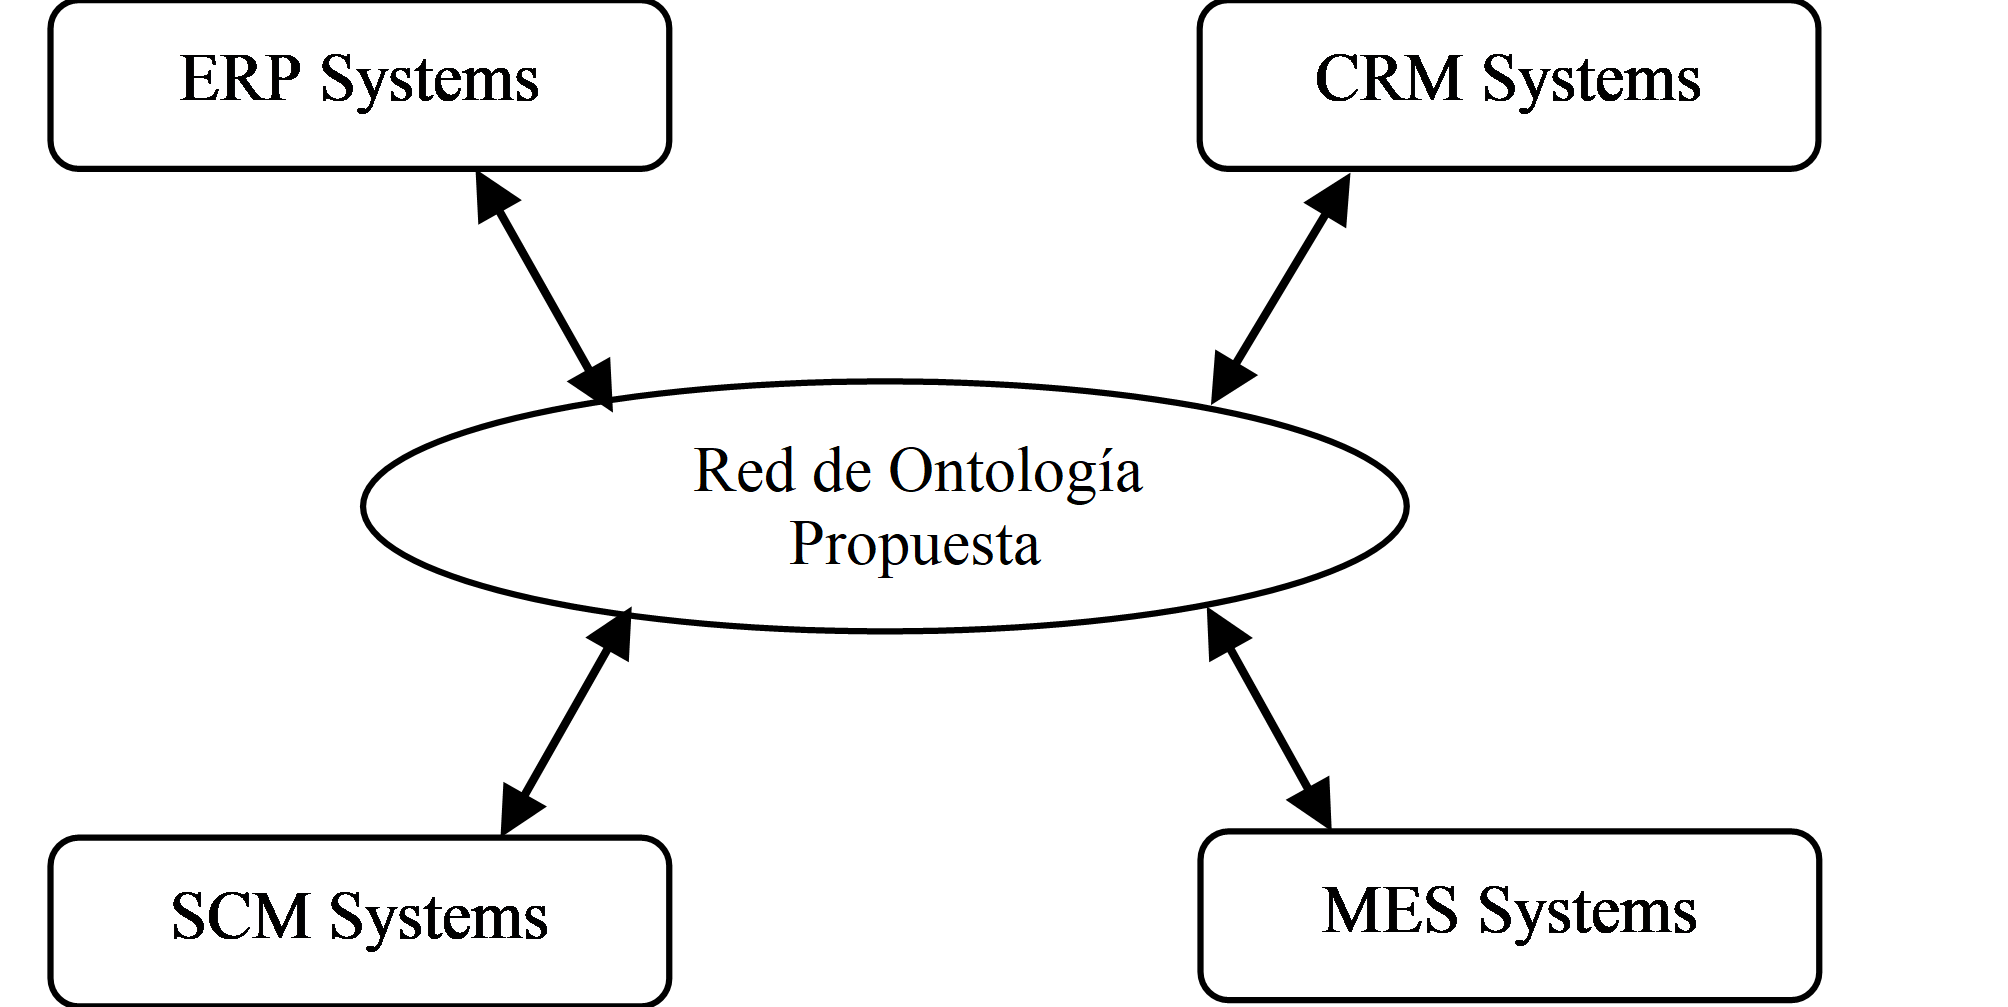
\includegraphics[width=3.5in]{figures/figure1.png}
\caption{Interoperabilidad Sem\'antica mediante la Red de Ontolog\'ia.}
\label{fig1}
\end{figure}

La arquitectura de la red de ontolog\'ia (\ref{fig2}) consta de varios niveles. Cada una de estas capas tiene un alcance, refiri\'endose al detalle que va refinando los t\'erminos m\'as importantes del ciclo de producto, ya sea de manera general o espec\'ifica a un est\'andar, modelo o vocabulario. Los niveles de la red son los siguientes:

\begin{itemize}
    \item Nivel Principal (Core Level): define un conjunto de t\'erminos considerados como claves en toda industria de manufactura.
    \item Nivel de Refinamiento (Refinement Level): contiene ontolog\'ias modulares que especifican un conjunto de t\'erminos comunes a varios est\'andares, que permiten refinar los conceptos definidos en la capa superior.
    \item Capa de Alineamiento (Inter-middle Alignment Level): proporciona las reglas de inferencia necesarias para igualar los t\'erminos introducidos en el nivel intermedio e inferior.
    \item Nivel de Est\'andares (Standards Level): agrupa un conjunto de ontolog\'ias que formalizan cada uno de los est\'andares y/o partes de est\'andares que por medio de reglas definidas en la capa de alineamiento permite la interoperabilidad entre las formalizaciones presentes en este nivel.  
\end{itemize}



\begin{figure}[!t]
\centering
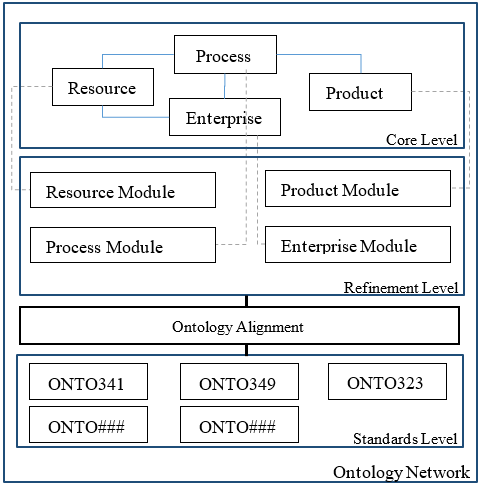
\includegraphics[width=3.5in]{figures/figure2.png}
\caption{Arquitectura de Tres Niveles de la Red de Ontolog\'ias Propuesta.}
\label{fig2}
\end{figure}



\subsubsection{Descripci\'on del Nivel Principal}

En la Figura \ref{fig3}, se observa el esquema conceptual del nivel principal ``Core Level". Compuesta por una ontolog\'ia que especifica cuatro t\'erminos: \emph{Process}, \emph{Product}, \emph{Resource} y \emph{Enterprise}. Estos t\'erminos son considerados por Zhao et al. \cite{Zhao1999}, Lin y Harding \cite{Lin2007},  Chungoora et al. \cite{Chungoora2013c} y Usman et al. \cite{Usman2013} como principales de toda industria de manufactura. A su vez, la figura señala las relaciones entre los t\'erminos y los est\'andares que los definen.

Se decidi\'o asociar los t\'erminos \emph{Product} y \emph{Process} a causa de la definici\'on de \emph{Process} en ISO 10303-49 \cite{ISOProperties}, la cual enuncia: ``Un procedimiento particular para hacer algo que involucra uno o m\'as pasos u operaciones. El proceso puede producir un producto, una propiedad de un producto o un aspecto de un producto". 

\begin{figure}[!t]
\centering
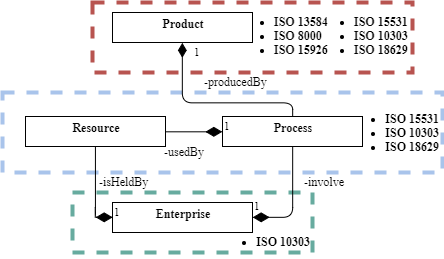
\includegraphics[width=3.5in]{figures/figure3.png}
\caption{Esquema Conceptual del nivel principal.}
\label{fig3}
\end{figure}

El t\'ermino \emph{Process} aparece relacionado a \emph{Enterprise} en los est\'andares ISO 15531 \cite{ISO2004} e ISO 18629 \cite{ISOPrinciplesc}. Ambos est\'andares describen a \emph{Process} como: ``Conjunto de actividades involucrando varias entidades empresariales que est\'an organizadas con un prop\'osito". Asimismo, \emph{Enterprise} es definido en ISO 100303-239, como una o m\'as organizaciones con un conjunto de metas y objetivos para ofrecer productos y/o servicios.

\subsubsection{Descripción del Nivel de Refinamiento}

El nivel de refinamiento posee cuatro ontolog\'ias individuales, que llamamos m\'odulos. Los m\'odulos tienen como funci\'on, especificar los t\'erminos que se ven fuertemente relacionados con los introducidos en el primer nivel, es decir, \emph{Process}, \emph{Product}, \emph{Resource} y \emph{Enterprise}, extendiendo as\'i, sus definiciones en la arquitectura.

Las Figuras \ref{fig4}, \ref{fig5}, \ref{fig6} y \ref{fig7} ilustran los diagramas que corresponden a cada uno de los m\'odulos de la capa de refinamiento de la arquitectura. Es preciso remarcar que estos m\'odulos no se encuentran aislados, sino que se relacionan por medio del t\'ermino del nivel principal, como se puede apreciar en las figuras. Esto permite mantener el contexto de las conceptualizaciones de los t\'erminos involucrados, es decir, que cada m\'odulo \'unicamente integra t\'erminos referentes al t\'ermino con el que se relaciona del nivel principal.

Los t\'erminos seleccionados para integrar cada m\'odulo son los que con frecuencia son mencionados a lo largo de los est\'andares publicados por el ISO TC184/SC4. Adem\'as, se puede mencionar la existencia de relaciones binarias entre t\'erminos de diferentes m\'odulos por medio de propiedades que se encuentran enunciadas en los est\'andares, este es el caso de \emph{Process\_Material}.

El m\'odulo del t\'ermino \emph{Process}, que se muestra en la Figura \ref{fig4} incluye los t\'erminos \emph{Natural\_Process}, \emph{Artificial\_Process}. Estos dos t\'erminos participan de la definici\'on de \emph{Product} en los est\'andares ISO 8000, ISO 10303, ISO 13584, ISO 15531, ISO 15926, ISO 18629. En la Figura \ref{fig4}, se observa que el t\'ermino \emph{Procedure} materializa al t\'ermino \emph{Process}, de acuerdo con su definici\'on en ISO 10303. Una \emph{Process\_Activity} es un paso u operaci\'on que forma parte de un \emph{Process} y \emph{Procedure\_Activity} es una ejecuci\'on espec\'ifica de un \emph{Process\_Activity}. El recurso requerido para ejecutar un \emph{Process\_Activity} se denomina \emph{Process\_Material}. El conjunto de procesos necesarios para fabricar un producto, est\'an vinculados por medio de un \emph{Process\_Plan}, el cual se ejecuta en una \emph{Process\_Plant}.

En la Figura \ref{fig5} se presenta el diagrama que corresponde al m\'odulo del t\'ermino \emph{Product}. En dicha figura se observa los t\'erminos \emph{Instruction}, \emph{Fact}, y \emph{Concept} como especializaciones de \emph{Product Information}. El t\'ermino \emph{Instruction} describe informaci\'on sobre c\'omo hacer o c\'omo usar algo, mientras que \emph{Fact} es la informaci\'on at\'omica del producto y \emph{Concept} es la noci\'on o idea acerca del mismo.

\begin{figure}[!t]
\centering
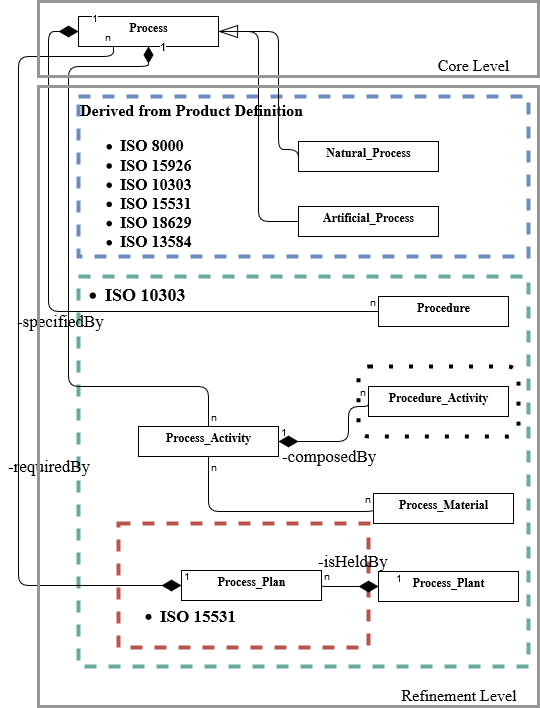
\includegraphics[width=3.5in]{figures/Completo-Process.png}
\caption{T\'erminos del M\'odulo \emph{Process}.}
\label{fig4}
\end{figure}

En el est\'andar ISO 10303-1, se mencionan dos definiciones para el t\'ermino \emph{Product}, una de ellas es la misma para \emph{Product Information}. En la propuesta se introduce el concepto \emph{Product\_Information} al m\'odulo de \emph{Product} y se lo asocia al concepto mediante la relaci\'on, \emph{definedBy}. Se observa en la figura que tambi\'en aparecen en el diagrama los t\'erminos \emph{Substance} y \emph{Thing} como subsunci\'on del t\'ermino \emph{Product}. Esta decisi\'on se fundamenta en que los est\'andares ISO 8000, ISO 10303, ISO 13584, ISO 15531, ISO 15926 y ISO 18629, definen a \emph{Product} como una cosa o sustancia producida por un proceso natural o artificial.

\begin{figure}[!t]
\centering
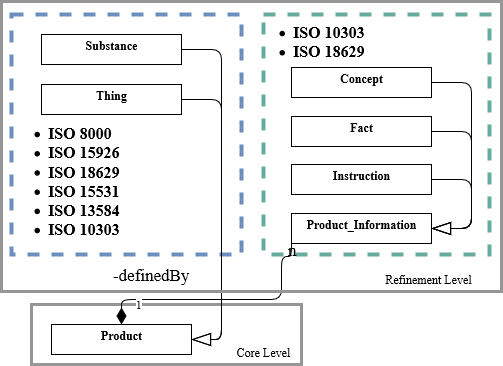
\includegraphics[width=3.5in]{figures/Completo-Product.png}
\caption{T\'erminos Pertenecientes al M\'odulo \emph{Product}.}
\label{fig5}
\end{figure}

El m\'odulo que refina el t\'ermino \emph{Resource} se introduce en la Figura \ref{fig6}. Seg\'un ISO 10303-49, un \emph{Resource} est\'a definido por sus comportamientos y capacidades, por lo que se asocia con los t\'erminos \emph{Behaviour} y \emph{Capability}. Asimismo, forman parte del m\'odulo los t\'erminos \emph{Tool}, \emph{Equip}, y \emph{Device}, que los est\'andares ISO 15531 e ISO 18629 describen como recursos. 

\begin{figure}[!t]
\centering
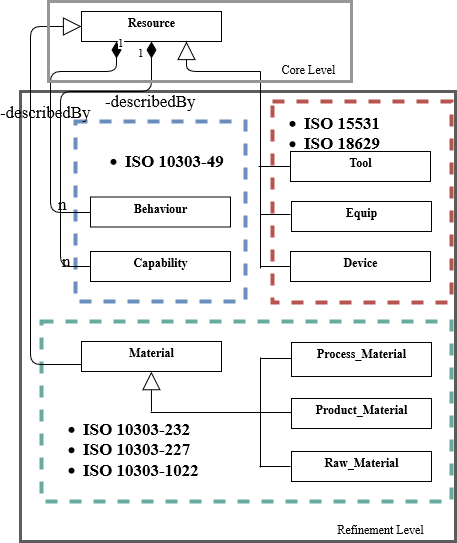
\includegraphics[width=3.5in]{figures/Completo-Resource.png}
\caption{T\'erminos del M\'odulo \emph{Resource}.}
\label{fig6}
\end{figure}

Otros est\'andares, agregan m\'as t\'erminos a esta relaci\'on de subsunci\'on del t\'ermino \emph{Resource}, como, por ejemplo: \emph{Procees\_Material} y \emph{Product\_Material}. Seg\'un ISO 10303-227, el primer t\'ermino, define el material usado o transportado por una actividad de proceso. En tanto, el segundo t\'ermino, se refiere, de acuerdo con el ISO 10303-235, al objeto f\'isico que fue fabricado seg\'un una especificaci\'on y del cual se puede fabricar otro producto. Teniendo en cuenta esto, se define una relaci\'on de subsunci\'on entre "Material" y los t\'erminos \emph{Product\_Material}, \emph{Process\_Material} y \emph{Raw\_Material}.

El m\'odulo del t\'ermino \emph{Enterprise} (Figura \ref{fig7}), es refinado usando el modelo de manufactura de cuatro niveles presente en \cite{Zhao1999}. Este modelo representa los niveles en los cuales un proceso o plan de proceso puede ser ejecutado e incluye desde la organizaci\'on hasta las estaciones de trabajo. Una estaci\'on de trabajo, \emph{Station}, es donde se realiza un trabajo en especial. El t\'ermino \emph{Cell} es un grupo de operaciones relacionadas en el flujo de producci\'on, mientras que \emph{Shop} es el \'area donde se lleva a cabo la producci\'on, y \emph{Factory} es el lugar donde se encuentran esas \'areas de producci\'on. A su vez, \emph{Enterprise} est\'a compuesta por un conjunto de \emph{Factory}.

\begin{figure}[!t]
\centering
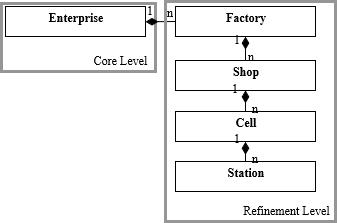
\includegraphics[width=3.5in]{figures/Completo-Enterprise.png}
\caption{T\'erminos Pertenecientes al M\'odulo \emph{Enterprise}.}
\label{fig7}
\end{figure}

\subsubsection{Descripci\'on del Nivel de Est\'andares}

En el nivel de est\'andares se agrupan las diferentes ontolog\'ias, implementadas en OWL, que formalizan los est\'andares, que van a interoperar, algunos de los cuales se encuentran mencionados previamente en las Tablas \ref{tabla1}, \ref{tabla2} y \ref{tabla3}. Es importante mencionar que tambi\'en se pueden incorporar otros tipos de modelos de datos de producto que no pertenezcan a los est\'andares publicados por el ISO TC184/SC4.  

A los modelos de datos integrados en este \'ultimo nivel se definen un conjunto de reglas de inferencia, definidas en el lenguaje de reglas sem\'anticas (SWRL) para establecer una correspondencia con los t\'erminos definidos en el nivel de refinamiento. Este conjunto de reglas de inferencias es tratado como una capa intermedia, que provee el enlace entre los niveles de refinamiento y de est\'andares. 


En la subsecci\'on siguiente se describe el como se llevo a cabo la implmentaci\'on de la red de ontolog\'ias y que tecnolog\'ias se han utilizado.

\subsection{Implementaci\'on}

La implementaci\'on de la red de ontolog\'ia se realiz\'o en OWL (Ontology Web Language) utilizando el editor Pr\'oteg\'e 5.2.0. El proceso comenz\'o por la codificaci\'on de todas ontolog\'ias por separado. El archivo principal conteniendo la ontolog\'ia del nivel principal de la red, fue llamado CoreConcepts.owl. Los archivos conteniendo las codificaciones de los m\'odulos que forman al nivel de refinamiento (Resourse, Product, Process y Enterprise) fueron llamados ResourceMod.owl, ProductMod.owl, ProcessMod.owl y EnterpriseMod.owl. 

Los m\'odulos del nivel de refinamiento: Product Module, Process Module, Resource Module y Enterprise Module, se encuentran implementados de manera aislada en el lenguaje OWL. Estas cuatro ontolog\'ias son importadas en la ontolog\'ia   principal para su uso. Los t\'erminos de nivel de refinamiento, a su vez se vinculan tanto de manera vertical como horizontal. Es decir, se encuentran propiedades que pueden vincular a las entidades de un m\'odulo con entidades de otro adyacente, como tambi\'en, con el t\'ermino principal que da nombre al m\'odulo. 

El nivel de est\'andares consta de un archivo codificado en OWL, por cada est\'andar adaptado. Estos archivos son importados en la ontolog\'ia principal, en conjunto con reglas SWRL necesarias para lograr un emparejamiento con los t\'erminos definidos en la capa de refinamiento.

Recapitulando, en esta secci\'on se ha presentado la red de ontolog\'ia, su arquitectura e implementaci\'on, como as\'i tambi\'en algunas preguntas de competencia en SPARQL que permiten validar la red, as\'i como obtener informaci\'on de las entidades. 



\subsection{Verificaci\'on de la Red de Ontolog\'ia}

Cuantificar la calidad de una ontolog\'ia puede dificultarse, debido a la ausencia de un método formal aceptado que tenga en cuenta todos los criterios (coherencia, concisi\'on, inteligibilidad, adaptabilidad, compromiso ontol\'ogico m\'inimo, etc.) que pueden aplicarse para evaluar las ontolog\'ias de dominio.

Seg\'un G\'omez-P\'erez \cite{Gomez-Perez2007OntologicalWeb}, la fase de evaluaci\'on ontol\'ogica comprende tres aspectos: i) validaci\'on ontol\'ogica, ii) verificaci\'on ontol\'ogica y iii) evaluaci\'on ontol\'ogica. Las actividades de validaci\'on y verificaci\'on est\'an asociadas con un juicio t\'ecnico del contenido de la ontolog\'ia con respecto a un marco de referencia, que est\'an asociadas a la especificaciones de requisitos, preguntas de competencia o el mundo real. La validaci\'on est\'a relacionada con el reflejo del dominio en la definici\'on y modelado de la ontolog\'ia, mientras que la verificaci\'on intenta probar que las definiciones de ontolog\'ia implementan correctamente los requisitos de ontolog\'ia, esto \'ultimo relacionado con las preguntas de competencia \cite{Bezerra2013EvaluatingQuestions}. A su vez, la evaluaci\'on se centra en juzgar el contenido de la ontolog\'ia desde el punto de vista del usuario y la aplicaci\'on de esta en el dominio para la que fue creada. 

Esta red de ontolog\'ia se verifica por cada integraci\'on que se realiza en el \'ultimo nivel por medio de las preguntas de competencia. Las preguntas de competencia se formalizaron empleando el lenguaje de consulta SPARQL normalizado por la W3C. La estructura para realizar dichas consultas consta de dos partes principales, delimitadas por el uso de palabras claves. La primera parte comienza con la declaraci\'on de la palabra clave SELECT, a continuaci\'on, se anexa los nombres de las variables que se desean que retorne la ejecuci\'on de la consulta. La segunda parte de estas consultas est\'a compuesta por la estructura que comienza con la palabra clave WHERE, en dicha porci\'on se debe detallar patrones de tripletas que se desean localizar dentro de la ontolog\'ia, aplicando tambi\'en los nombres de las variables que se desean devolver por la porci\'on delimitada por la palabra clave SELECT. 

Otras secciones pueden ser declaradas dentro de la consulta mediante el uso de otras palabras claves, por ejemplo, la palabra clave FILTER, dicha palabra clave permite separar subconjuntos de tripletas utilizando condiciones l\'ogicas o expresiones regulares. 

En la Tabla \ref{tabla4}, la primera fila muestra la pregunta ``¿Qu\'e recursos necesita el proceso X?". Esta pregunta puede ser transformada en un equivalente en SPARQL, la cual se presenta en la segunda columna de la misma fila. La consulta devuelve la variable \emph{?resource}, que es usada en el patr\'on de tripletas declarado por la porci\'on de la palabra clave WHERE, que indica que dicha variable se encuentra relacionada, a trav\'es de la propiedad \emph{tc:usedBy} con otra variable denominada \emph{?process}, la que es empleada en la \'ultima porci\'on de la consulta para buscar coincidencias de palabras ingresada en la funci\'on \emph{regex}, la cual es aplicada para definir expresiones regulares y as\'i filtrar resultados de las tripletas identificadas. Resumiendo, lo que esta consulta devuelve son los individuos que est\'en relacionados por la propiedad \emph{tc:usedBy}, con determinados valores de cadena de caracteres en la variable \emph{?process}.

La siguiente pregunta ``¿Qu\'e recursos son necesarios para ejecutar un plan de proceso?", tiene como prop\'osito retornar los recursos que se ven involucrados a lo largo de un plan de proceso. Esta se diferencia de la anterior en que devuelve todos los recursos involucrados en el conjunto de procesos asociados a un plan determinado. Al igual que la consulta anterior, se puede escribir un equivalente en SPARQL para ejecutarla sobre la base de conocimiento. La misma emplea una variable de retorno que representa a los individuos del t\'ermino \emph{Resource} asociados, por medio de la propiedad \emph{tc.usedBy}, con el t\'ermino \emph{Process}. A su vez se declara el patr\'on de tripleta que relaciona a los individuos del t\'ermino \emph{Process}, representados por la variable \emph{?process}, con los individuos del t\'ermino \emph{Process\_Plan}, representados por la variable \emph{?process\_plan}, por \'ultimo, se declara un filtro para definir, como en el caso anterior, el nombre del plan de proceso del cual se desean conocer los recursos para su ejecuci\'on.

La \'ultima pregunta de la Tabla \ref{tabla4}, ``¿Qu\'e productos hacen uso de un recurso X?", retorna los productos, mediante la declaraci\'on de la variable \emph{?product}, que a lo largo de su proceso de fabricaci\'on necesitan o requieren de un respectivo recurso, que es representado por la variable \emph{?resource}, la que en la consulta presentada posee un filtro para identificar ese recurso necesario.


A continuaci\'on, se describe el proceso para incorporar nuevas ontolog\'ias a este nivel de la arquitectura. 

\subsection{Extensi\'on de la red propuesta mediante la incorporaci\'on de nuevos modelos de datos}

El proceso de incorporaci\'on es importante en la presente propuesta debido a la flexibilidad que aporta a la red de ontolog\'ias. Esta red es capaz de proveer mediaci\'on entre diferentes modelos de datos del dominio de la manufactura, no tan solo aquellos est\'andares que forman parte del comit\'e t\'ecnico 184 subcomit\'e 4, sino que adem\'as se pueden incorporar vocabularios, modelos, est\'andares que no pertenezcan al mencionado comit\'e simplemente agregando su formalizaci\'on en OWL en el \'ultimo nivel de la red. 


El proceso de integraci\'on de nuevo modelos de datos a la Red, comienza seleccionando el est\'andar, lenguaje, vocabulario o modelo que necesita ser integrado con otros est\'andares ya incorporados a la red. Una vez realizada esta selecci\'on, se identifican las fuentes de informaci\'on que se utilizar\'an para desarrollar la ontolog\'ia. Estas fuentes de informaci\'on pueden ser ontol\'ogicas o no ontol\'ogicas. Dentro de las ontol\'ogicas, es posible destacar diversas contribuciones por parte de la academia de ontolog\'ias basadas en est\'andares o modelos.

Por otro lado, las fuentes no ontol\'ogicas representan los documentos que describen las conceptualizaciones de t\'erminos, relaciones y restricciones entre t\'erminos. Las normas publicadas por el ISO TC186/SC4 se encuentran en esta categor\'ia. 

Una vez identificadas este tipo de fuentes, son estudiadas y analizadas para construir una nueva ontolog\'ia a partir de ellas. Un proceso semiautom\'atico para la adaptaci\'on de estos documentos en ontolog\'ias codificadas en OWL, ha sido propuesto por los autores en \cite{Fraga2017}, pero su descripci\'on est\'a fuera del alcance del presente art\'iculo. La ontolog\'ia obtenida como resultado de dicho proceso es, entonces, estudiaba para fusionarla con las extra\'idas de las fuentes ontol\'ogicas pudiendo completar y mejorar las definiciones de los t\'erminos presentes en la primera.

Una vez realizada la actividad de fusi\'on de ontolog\'ias, se la somete a una evaluaci\'on. Se proponen dos herramientas diferentes para esta actividad. El primero es OOPS! Scanner \cite{Poveda-Villalon2009a}, el cual se emplea para encontrar errores de diseño comunes y verificar la consistencia de la ontolog\'ia. La segunda consiste en usar preguntas de competencia escritas en el lenguaje de consulta SPARQL para verificar si cumple los requisitos establecidos para la incorporaci\'on de la nueva ontolog\'ia. Si la ontolog\'ia pasa ambas pruebas, se importa a la red ontol\'ogica como parte de su nivel de est\'andares.

A continuaci\'on, se definen un conjunto de reglas SWRL para alinear la nueva ontolog\'ia incorporada con los conceptos ya definidos por la red. Luego, la red actualizada es verificada utilizando una vez m\'as las preguntas de competencia. Estas preguntas fueron definidas en la fase de educci\'on de requisitos de la red de ontolog\'ia, algunas de las mismas se pueden apreciar en la Tabla \ref{tabla4}.


\begin{table}[!t]
\renewcommand{\arraystretch}{1.3}
\caption{Preguntas de Inferencia en SPARQL}
\label{tabla4}
\centering
\begin{tabular}{p{3cm}p{5cm}}
\hline
\hline
 Pregunta &  Consulta \\
\hline
¿Qu\'e recursos necesita el proceso X? & SELECT ?resource WHERE {?resource tc:usedBy ?process. FILTER regex(str(?process), ``\textless process\_name \textgreater \$")} \\ \cline{1-2}
¿Qu\'e recursos son necesarios para ejecutar un plan de proceso? &  SELECT ?resourse WHERE {?resource tc:usedBy ?process.
?process tc:requiredBy ?process\_plan FILTER regex (str(?process\_plan), ``\textless product\_name \textgreater \$")}  \\ \cline{1-2}
¿Qu\'e productos hacen uso de un recurso X? &  SELECT ?resource WHERE {
?process tc:requiredBy ?process\_plan. 
?process tc:produce ?product. 
?resource tc:usedBy ?process.
FILTER regex(str(?product),``\textless resource\_name \textgreater \$")}  \\  \hline \hline                                                                                                    
\end{tabular}
\end{table}

En la siguiente secci\'on se ilustra c\'omo se incorporan dos est\'andares, uno del comit\'e ISO mencionado y otro que no pertenece al mismo, a la red de ontolog\'ias. Con este caso de estudio, se evidencia la utilidad de la red propuesta para interoperar sistemas que implementen o hagan uso de los est\'andares del ISO TC184/SC4, as\'i como tambi\'en para abordar problemas de interoperabilidad entre distintos sistemas industriales que no utilicen est\'andares ISO.


\section{Caso de estudio}

En esta secci\'on se presenta un caso de estudio, en el cual se pone a prueba la red de ontolog\'ia mostrando su alcance, validez y utilidad mediante la incorporaci\'on del est\'andar ISO 10303-49 y el lenguaje de modelado de procesos IDEF3 a la red propuesta.

En la Figura \ref{fig8} se muestra un esquema gen\'erico, ilustrando el rol y la funci\'on de mediador que ejerce la red de ontolog\'ia entre los dos sistemas que implementan cada uno de los modelos. A partir de estos sistemas se obtendr\'an los individuos que poblar\'an las diferentes ontolog\'ias que tienen la red propuesta. Uno de los sistemas basado en IDEF3 y el otro adhiere al est\'andar ISO 10303-49.

\begin{figure}[!t]
\centering
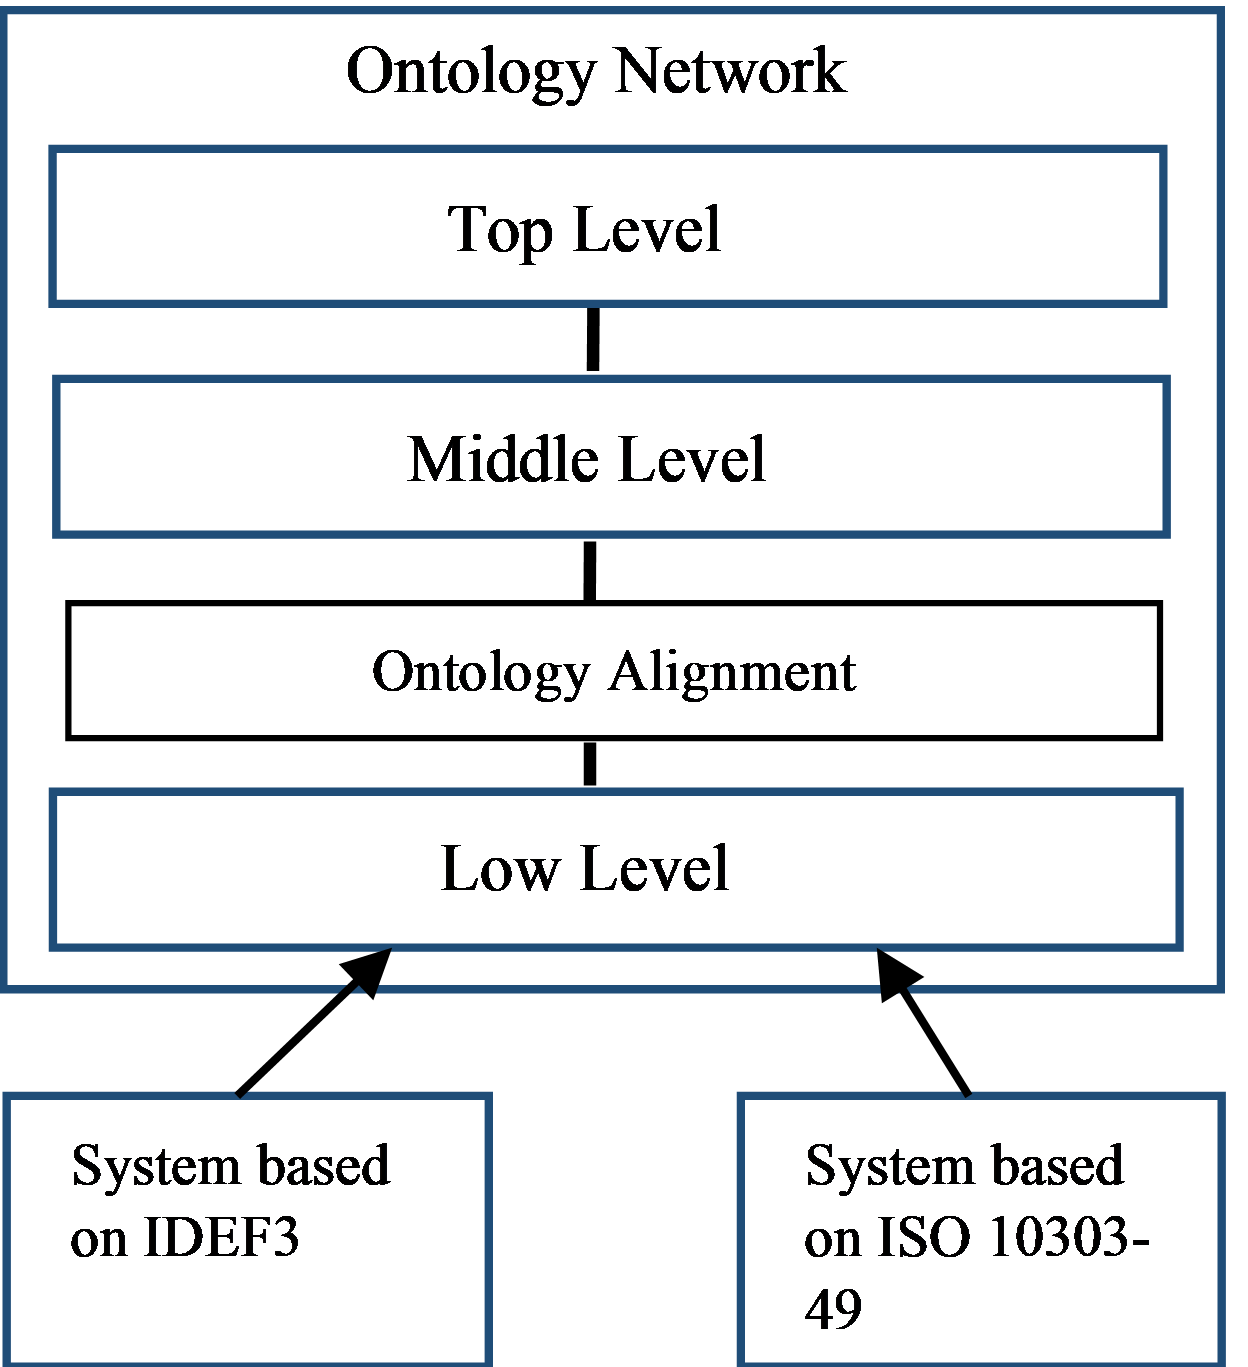
\includegraphics[width=3.5in]{figures/figure8.png}
\caption{Componentes del Caso de Estudio.}
\label{fig8}
\end{figure}

Como primer paso para lograr la integraci\'on sem\'antica de estos dos sistemas, es necesaria la creaci\'on e instanciaci\'on de las ontolog\'ias que formalicen los conceptos de IDEF3 y de ISO 10303-49, que ser\'an incorporadas al nivel inferior de la red. Asimismo, es necesario la definici\'on de un componente de alineamiento entre estas nuevas ontolog\'ias agregadas al nivel inferior y los conceptos pertenecientes a los otros niveles de la red propuesta. 

El est\'andar ISO 10303 parte 49 define la estructura para especificar: relaciones entre los procesos, la efectividad de un proceso, las propiedades de un proceso, los recursos necesarios para el proceso, las propiedades del recurso, la representaci\'on del proceso, la representaci\'on del recurso, y la relaci\'on del proceso con los productos. 

La Tabla \ref{tabla5} y la Figura \ref{fig9} ilustran la definici\'on de algunos t\'erminos m\'as importantes pertenecientes a ISO 10303-49 y sus relaciones. Los t\'erminos listados en dicha tabla no son todos los t\'erminos definidos por la norma, pero son los empleados en esta secci\'on para mostrar la interacci\'on de las ontolog\'ias integradas


\begin{figure}[!t]
\centering
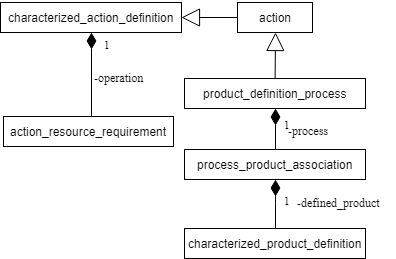
\includegraphics[width=3.5in]{figures/figure9.png}
\caption{Fragmento de ISO 10303-49.}
\label{fig9}
\end{figure}

\begin{table}[!t]
\renewcommand{\arraystretch}{1.3}
\caption{T\'erminos y definiciones ISO 10303-49}
\label{tabla5}
\centering
\begin{tabular}{cp{4cm}}
\hline
\hline
 T\'erminos ISO 10303-49 &  Definiciones \\
\hline
Action\_resource\_requirement & Define los recursos requeridos para un proceso. \\ \cline{1-2}
Product\_definition\_process & Representa la definici\'on de un producto, un producto o un aspecto de este. \\ \cline{1-2}
Process\_product\_association & Especifica un proceso que lleva a cabo una caracter\'istica especifica de un producto. \\  \cline{1-2}
Characterized\_product\_definition & Define las caracter\'isticas de un proceso. \\
\hline \hline
\end{tabular}
\end{table}

La Tabla \ref{tabla6}, muestra un extracto de tres reglas que han sido definidas para alcanzar la interoperabilidad entre el m\'odulo del est\'andar ISO 10303-49, formalizado en una ontolog\'ia OWL, que ha sido incorporada previamente en el \'ultimo nivel de la red, con las otras ontolog\'ias de la red propuesta. Estas reglas describen c\'omo los individuos del m\'odulo pueden ser inferidos, con la ayuda de un razonador, como individuos de los conceptos de los diferentes niveles de la red de ontolog\'ias.

\begin{table}[!t]
\renewcommand{\arraystretch}{1.3}
\caption{Reglas de mapeo entre ISO 10303-49 y la red de ontolog\'ias}
\label{tabla6}
\centering
\begin{tabular}{p{2.5cm}p{5cm}}
\hline
\hline
 Nombre &  Regla \\
\hline
R\_Process & \begin{verbatim}characterized_action_
definition(?x) ^ 
action_schema_action(?x) ^ 
product_definition_process(?x) 
-> Process(?x) \end{verbatim}  \\ \cline{1-2}
R\_Resource & \begin{verbatim}characterized_action_
definition(?y) ^ 
operation(?x, ?y) ^ 
action_schema_action(?y) ^ 
action_resource_
requirement(?x) ^ 
product_definition_
process(?y) -> 
usedBy(?x, ?y) ^ 
Process(?y) ^ 
Process_Material(?x) \end{verbatim} \\ \cline{1-2}
R\_Process\_Activity & \begin{verbatim}characterized_action_
definition(?y) ^ 
action_schema_action(?y) ^ 
product_definition_
process(?y) ^ 
process_product_association_
process(?x, ?y) -> 
Process_Activity(?x) ^ 
Process(?y) ^ 
composedBy(?x,?y) \end{verbatim} \\  \hline \hline   
\end{tabular}
\end{table}

La regla cuyo nombre es R\_Process espec\'ifica que si X es un individuo en la poblaci\'on del concepto \emph{product\_definition\_process}, entonces, X es un individuo de la entidad \emph{Process} en el nivel principal. La regla R\_Resource detalla que si X es un \emph{action\_resource\_requirement} y est\'a relacionado con Y, a trav\'es de la propiedad \emph{operation}, entonces, X es un \emph{Process\_Material}, t\'ermino presente en el nivel de refinamiento. Dado que el concepto \emph{Process\_Material} es una especializaci\'on de la clase \emph{Resource} (Fig. \ref{fig6}), X es tambi\'en instancia de dicha clase. Asimismo, el individuo Y del tipo \emph{characterized\_action\_definition} es definido como instancia de tipo \emph{Process\_Activity}. Estas instancias definen actividades at\'omicas que hacen uso de los recursos en un proceso. Finalmente, la regla R\_Process\_Activity puntualiza que si X es un \emph{process\_product\_association} y est\'a relacionado con un individuo Y de la entidad \emph{product\_definition\_process} por la propiedad \emph{process\_product\_association\_process}, entonces, X es un \emph{Process\_Activity} e Y es el equivalente a \emph{Process} relacionados, a trav\'es de la propiedad \emph{composedby} en la red de ontolog\'ias. 

Por otra parte, IDEF3 es un lenguaje de modelado de procesos de negocios, captura de restricciones, requerimientos de cada acci\'on involucrada en el sistema incluyendo su temporalidad. 

El t\'ermino, unidad de comportamiento (UOB), en IDEF3, hace referencia al bloque que representa una actividad. M\'ultiples bloques de actividades se relacionan entre s\'i mediante los enlaces temporales (TemporalLink) con asociaciones que pueden especificarse para determinar si una actividad es predecesora o sucesora a una anexada con esta \'ultima. 

Para representar la divergencia o convergencia de los procesos, se utilizan las uniones o cruces. Estas pueden ser de ejecuci\'on en paralelo (AndJunction) o alternativo (OrJunction o XORJunction). As\'i tambi\'en, las ramificaciones de los caminos de ejecuci\'on pueden ser asincr\'onicas o sincr\'onicas. Los UOB pueden interactuar con objetos que pueden ser entradas (InputObject) o salidas (OutputObject) de los nodos de procesos. 

Como bien se ha presentado en la secci\'on anterior, la red de ontolog\'ia para poder incorporar nuevas adaptaciones funcionales necesita de una transformaci\'on del modelo a una ontolog\'ia codificada en OWL y de un conjunto de reglas definidas en SWRL.

En la Tabla \ref{tabla7} se muestran las entidades que est\'an involucradas en el caso de estudio por parte del sistema basado en IDEF3 y las entidades de la red de ontolog\'ias que ser\'an empleadas en la conformaci\'on de las reglas para la alineaci\'on.

\begin{table}[!t]
\renewcommand{\arraystretch}{1.3}
\caption{T\'erminos involucrados en el caso de estudio}
\label{tabla7}
\centering
\begin{tabular}{cp{4cm}}
\hline
\hline
IDEF3 &  Refinement Level \\ \hline
UOB & Process\_Activity \\ \cline{1-2}
TemporalLink & N/A \\ \cline{1-2}
InputObject & Resource - Process\_Material \\ \hline   
OutputObject & Product - Product\_Material \\ \hline
AndJunctionSynchronous & N/A \\ 
\hline \hline
\end{tabular}
\end{table}

Una vez obtenida la adaptaci\'on del modelo IDEF3, se importa la ontolog\'ia a la red y se procede a generar las reglas SWRL empleadas para lograr el alineamiento entre los t\'erminos de la ontolog\'ia que formaliza IDEF3 y los conceptos ya definidos en la red. La Tabla \ref{tabla8}, ilustra algunas de estas reglas.

\begin{table}[!t]
\renewcommand{\arraystretch}{1.3}
\caption{Reglas SWRL para alineamiento entre IDEF3 y la red de ontologias}
\label{tabla8}
\centering
\begin{tabular}{|c|p{6cm}|}
\hline
 Nombre &  Regla \\ \hline
UOB          & \begin{verbatim}UOB(?x) -> Process_Activity(?x) \end{verbatim} \\ \cline{1-2}
TemporalLink & \begin{verbatim}Input_Object(?x) ^ 
IDEF3_to(?x, ?y) ^ 
UOB(?y) -> usedBy(?x, ?y) ^ 
Process_Material(?x) ^ 
Process_Activity(?y) \end{verbatim} \\ \cline{1-2}
InputObject  & \begin{verbatim}UOB(?y) ^ 
IDEF3_from(?x, ?y) ^ 
Output_Object(?x) -> 
generatedBy(?x, ?y) ^  
Product_Material(?x) ^ 
Process_Activity(?y) \end{verbatim} \\ \hline   
\end{tabular}
\end{table}

La regla R\_UOB, señala que, si existe un individuo X que es instancia de \emph{UOB} entonces, X es instancia de \emph{Process\_Activity}. Se observa tambi\'en en la mencionada tabla las reglas R\_Input y R\_Output para los objetos de entrada y salida, respectivamente, de las UOB de IDEF3. R\_Input especifica que, si X es un individuo de la entidad \emph{Input\_Object} e Y es un \emph{UOB} asociados por la propiedad \emph{IDEF3\_to}, entonces, X es un \emph{Process\_Material} que se encuentra relacionado con la propiedad \emph{usedBy} con un individuo de la entidad \emph{Process\_Activity}. Por \'ultimo, la regla R\_Output especifica que, si X es un \emph{Output\_Object} e Y un \emph{UOB}, estos dos t\'erminos se asocian por la propiedad \emph{IDEF3\_from}, entonces, X es un individuo del t\'ermino \emph{Product\_Material} relacionado con un individuo Y que es un \emph{Process\_Activity}, por la propiedad \emph{generatedBy}.

El ejemplo elegido para este caso es el proceso de agregado de ingredientes para la producci\'on de pasta dental en gel. Como se observa en la figura \ref{fig10}, el mismo es representado utilizando los conceptos de IDEF3 y, como se ver\'a m\'as adelante en esta secci\'on, ser\'a consultado mediante los conceptos de ISO 10303-49. Este proceso consta de 4 operaciones: \emph{Add Water}, \emph{Add Fillers}, \emph{Add Stabilizers} y \emph{Add Soium Fluoride}. Estas operaciones son representadas por UOBs en IDEF3. \emph{Add Fillers} y \emph{Add Stabilizers} son operaciones que se realizan en paralelo caracterizadas por el uso del conector \emph{And}. Por \'ultimo, las operaciones se unen mediante un conector \emph{And} y termina con la \'ultima unidad llamada \emph{Add Sodium Fluoride}, la cual entrega un objeto salida para la siguiente etapa, llamado \emph{Mixture} al proceso \emph{React} del plan de proceso de fabricaci\'on de la pasta dental.

La Figura \ref{fig11} muestra diferentes vistas capturadas del editor Prot\'eg\'e. En particular, se observan: la vista de instancias correspondiente a la entidad \emph{Input\_Object} (parte izquierda de la figura); la vista de descripci\'on de individuo (parte superior derecha); y la vista de aserci\'on de propiedades de objetos. En estas dos \'ultimas vistas, se puede visualizar en fuente negrita los tipos definidos de manera expl\'icita. En tanto, los tipos que son inferidos, cuando se activa un razonador, en fuente normal con un sombreado color amarillo.  Las tres vistas que se presentan corresponden a la definici\'on del individuo \emph{Filler}, el cual ha sido definido expl\'icitamente como un \emph{Input\_Object} e inferido como un individuo del tipo \emph{action\_resource\_requirement} y \emph{Process\_Material}, estos dos \'ultimos t\'erminos mencionados son conceptos definidos en el est\'andar 10303-49 y la red propuesta, respectivamente. Asimismo, se observa que la propiedad de objeto \emph{usedBy} que asocia \emph{Filler} con la instancia \emph{Add\_Fillers} es inferida. La figura mencionada muestra como individuos definidos en IDEF3, pueden ser tratados como conceptos del est\'andar ISO 10303-49 y de la red de ontolog\'ias.


\begin{figure}[!t]
\centering
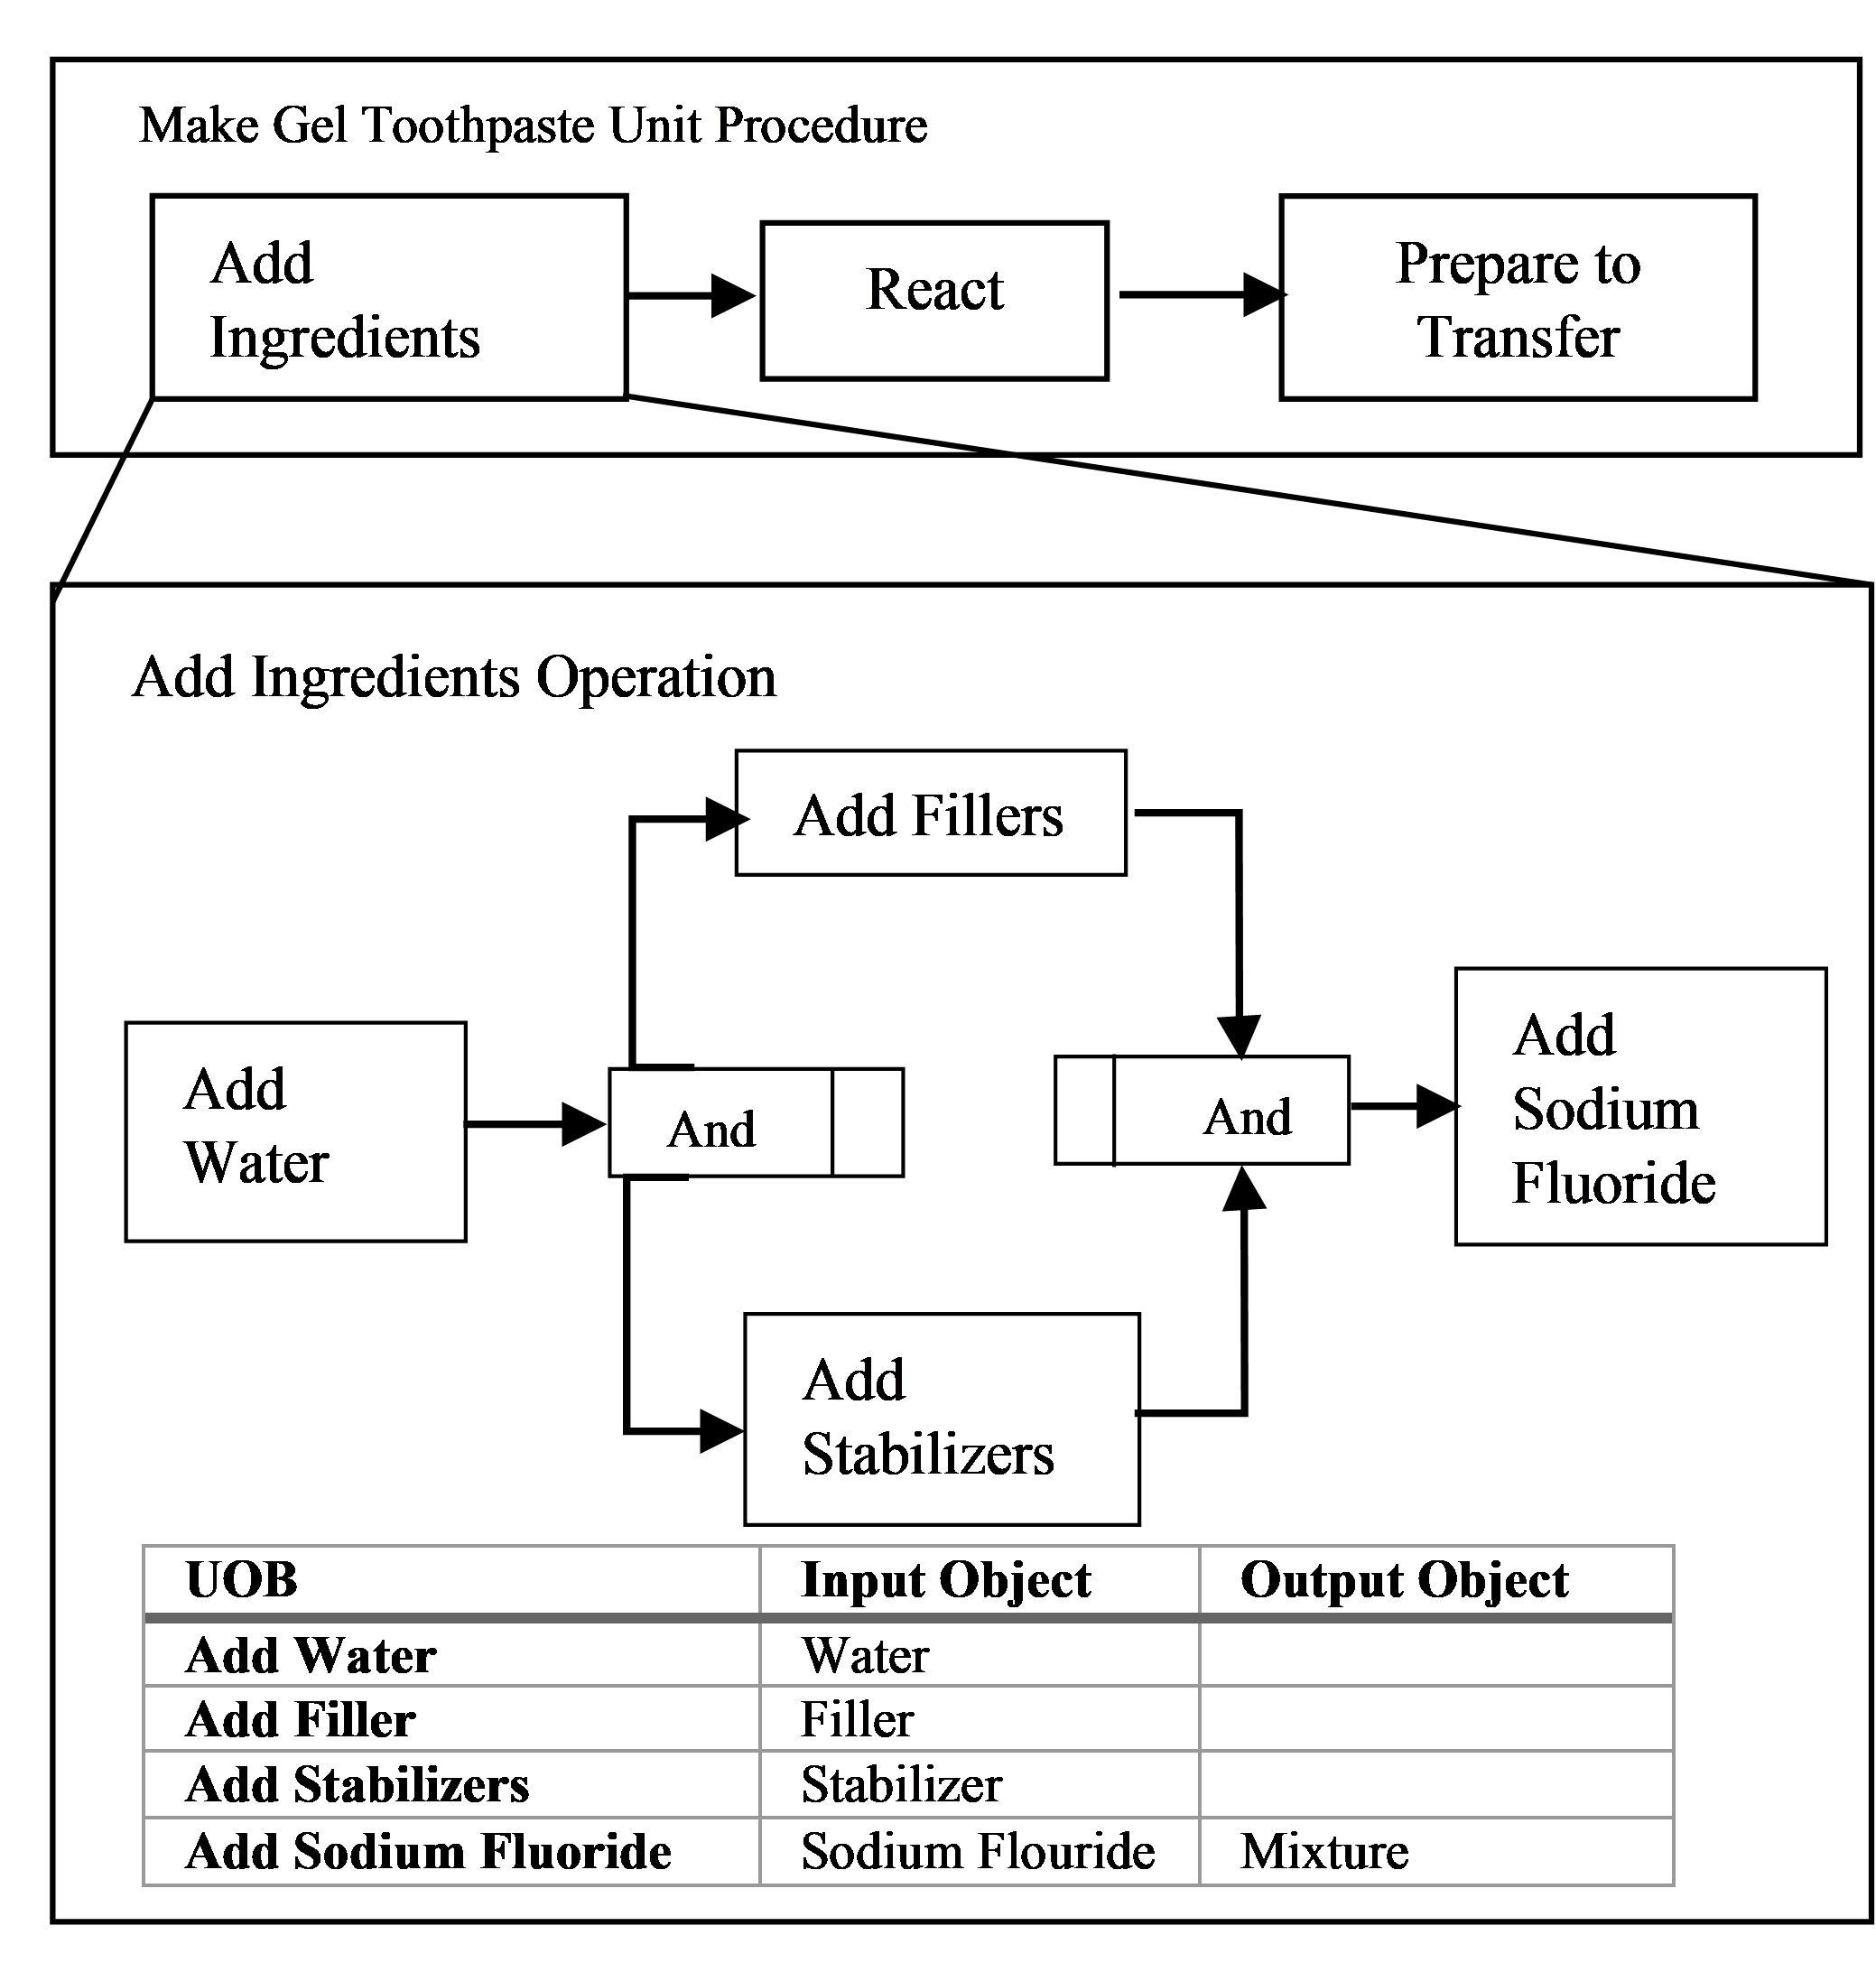
\includegraphics[width=3.5in]{figures/figure10.png}
\caption{Ejemplo del subproceso ``Add Ingredients Operation" del proceso principal ``Make Gel Toothpaste" en IDEF3.}
\label{fig10}
\end{figure}

\begin{figure}[!t]
\centering
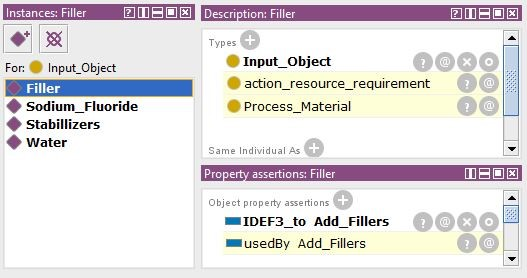
\includegraphics[width=3.5in]{figures/figure11.jpg}
\caption{Individuos del Caso de Estudio en Prot\'eg\'e.}
\label{fig11}
\end{figure}

Para inferir nuevos conocimientos y hacer uso de la red de ontolog\'ias y sus individuos, es posible generar distintas preguntas. Dichas preguntas pueden ser representadas mediante lenguajes de consulta. Es posible utilizar el lenguaje SPARQL sobre un SPARQL endpoint o utilizar el lenguaje Description Logic en la pestaña DL en Proteg\'e. El uso de este mecanismo sobre la red de ontolog\'ias demuestra su usabilidad. 

Como ejemplo considere las Figuras \ref{fig12} y \ref{fig13}. La Figura \ref{fig12}, presenta una consulta ingresada en la pestaña DL de Prot\'eg\'e que retorna las instancias del t\'ermino \emph{Resource}. En esta figura es posible ver como el individuo \emph{Filler}, que ha sido definido expl\'icitamente como instancia de \emph{Input\_Object} (Figura \ref{fig11}) es inferido como una instancia de \emph{Resource} (t\'ermino del nivel principal de la red de ontolog\'ias).


\begin{figure}[!t]
\centering
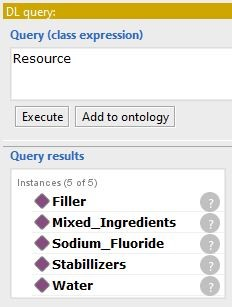
\includegraphics[width=3.5in]{figures/figure12.jpg}
\caption{Individuos representantes del t\'ermino ``Resource" a trav\'es de una consulta DL.}
\label{fig12}
\end{figure}

En tanto, la Figura \ref{fig13} presenta los individuos obtenidos como resultado de una consulta SPARQL que corresponde a la formalizaci\'on de la pregunta de competencia: ``¿Qu\'e recursos necesita el proceso ‘Add\_Ingredient’?". Es posible ver en dicha figura una lista de individuos del tipo \emph{Resource}, necesarios para el proceso denominado \emph{Add\_Ingredient}.

\begin{figure}[!t]
\centering
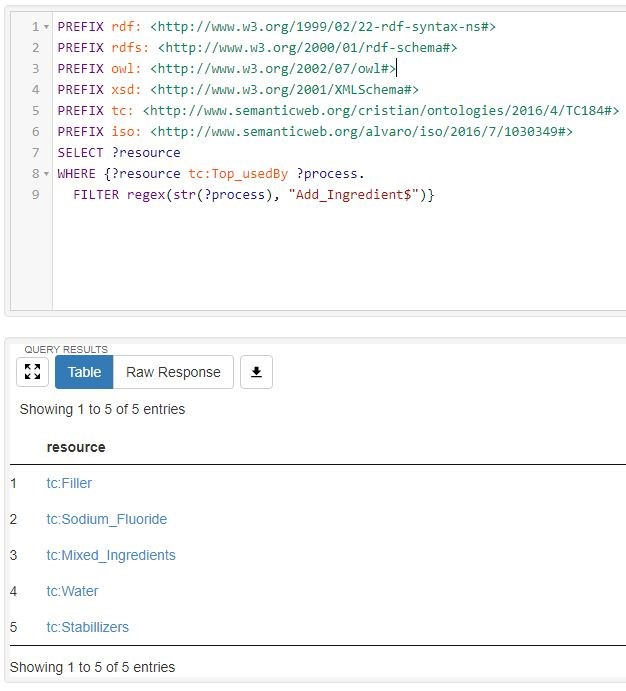
\includegraphics[width=3.5in]{figures/figure13.jpg}
\caption{Resultado de la ejecuci\'on de pregunta de competencia ``¿Qu\'e recursos necesita el proceso ‘Add\_Ingredient’?".}
\label{fig13}
\end{figure}


En esta \'ultima secci\'on hemos presentado la incorporación a la red propuesta de dos modelos de datos de productos, permitiendo que ambos modelos interoperen. Los dos modelos en cuesti\'on son, uno basado en el est\'andar ISO 10303-49 del comit\'e t\'ecnico 184 subcomit\'e y el otro del lenguaje de modelado IDEF3 y es posible observar que  la interoperbilidad es alcanzada por medio de la red de ontolog\'ias pudiendo \'esta inferir las clases a las cuales las instancias pertenecen y permitiendo dar respuesta a las preguntas de competencia planteadas en la tabla \ref{tabla4}. La respuesta a una de estas preguntas para el caso de estudio propuesto se muestra en la figura \ref{fig13}.

% An example of a floating figure using the graphicx package.
% Note that \label must occur AFTER (or within) \caption.
% For figures, \caption should occur after the \includegraphics.
% Note that IEEEtran v1.7 and later has special internal code that
% is designed to preserve the operation of \label within \caption
% even when the captionsoff option is in effect. However, because
% of issues like this, it may be the safest practice to put all your
% \label just after \caption rather than within \caption{}.
%
% Reminder: the "draftcls" or "draftclsnofoot", not "draft", class
% option should be used if it is desired that the figures are to be
% displayed while in draft mode.
%
%\begin{figure}[!t]
%\centering
%\includegraphics[width=2.5in]{myfigure}
% where an .eps filename suffix will be assumed under latex, 
% and a .pdf suffix will be assumed for pdflatex; or what has been declared
% via \DeclareGraphicsExtensions.
%\caption{Simulation results for the network.}
%\label{fig\_sim}
%\end{figure}

% Note that the IEEE typically puts floats only at the top, even when this
% results in a large percentage of a column being occupied by floats.


% An example of a double column floating figure using two subfigures.
% (The subfig.sty package must be loaded for this to work.)
% The subfigure \label commands are set within each subfloat command,
% and the \label for the overall figure must come after \caption.
% \hfil is used as a separator to get equal spacing.
% Watch out that the combined width of all the subfigures on a 
% line do not exceed the text width or a line break will occur.
%
%\begin{figure*}[!t]
%\centering
%\subfloat[Case I]{\includegraphics[width=2.5in]{box}%
%\label{fig\_first\_case}}
%\hfil
%\subfloat[Case II]{\includegraphics[width=2.5in]{box}%
%\label{fig\_second\_case}}
%\caption{Simulation results for the network.}
%\label{fig\_sim}
%\end{figure*}
%
% Note that often IEEE papers with subfigures do not employ subfigure
% captions (using the optional argument to \subfloat[]), but instead will
% reference/describe all of them (a), (b), etc., within the main caption.
% Be aware that for subfig.sty to generate the (a), (b), etc., subfigure
% labels, the optional argument to \subfloat must be present. If a
% subcaption is not desired, just leave its contents blank,
% e.g., \subfloat[].


% An example of a floating table. Note that, for IEEE style tables, the
% \caption command should come BEFORE the table and, given that table
% captions serve much like titles, are usually capitalized except for words
% such as a, an, and, as, at, but, by, for, in, nor, of, on, or, the, to
% and up, which are usually not capitalized unless they are the first or
% last word of the caption. Table text will default to \footnotesize as
% the IEEE normally uses this smaller font for tables.
% The \label must come after \caption as always.
%
%\begin{table}[!t]
%% increase table row spacing, adjust to taste
%\renewcommand{\arraystretch}{1.3}
% if using array.sty, it might be a good idea to tweak the value of
% \extrarowheight as needed to properly center the text within the cells
%\caption{An Example of a Table}
%\label{table\_example}
%\centering
%% Some packages, such as MDW tools, offer better commands for making tables
%% than the plain LaTeX2e tabular which is used here.
%\begin{tabular}{|c||c|}
%\hline
%One & Two\\
%\hline
%Three & Four\\
%\hline
%\end{tabular}
%\end{table}


% Note that the IEEE does not put floats in the very first column
% - or typically anywhere on the first page for that matter. Also,
% in-text middle ("here") positioning is typically not used, but it
% is allowed and encouraged for Computer Society conferences (but
% not Computer Society journals). Most IEEE journals/conferences use
% top floats exclusively. 
% Note that, LaTeX2e, unlike IEEE journals/conferences, places
% footnotes above bottom floats. This can be corrected via the
% \fnbelowfloat command of the stfloats package.




\section{Conclusi\'on}

Este trabajo presenta una red de ontolog\'ias multinivel, como soluci\'on al problema de interoperabilidad de sistemas heterog\'eneos que implementan los est\'andares del comit\'e 184 subcomit\'e 4 de la Organizaci\'on Internacional de Est\'andares. 

La ventaja principal de esta red, adem\'as de permitir interoperar con modelos implementados del mencionado comit\'e de la ISO puede ser extendida y usada para otros est\'andares y modelos de informaci\'on. Esto se logra agregando la formalizaci\'on del modelo requerido y las reglas necesarias para el alineamiento de las ontolog\'ias participantes. Pudiendo servir esta red de ontologias como mediador entre sistemas heterog\'eneos. Por esta raz\'on los sistemas inform\'aticos que se encuentren en cada industria no necesitar\'an efectuar cambios en su estructura. Solo se requeriria la formalizacion de los modelos de datos utilizando OWL y la definicion de las correspondiente reglas de inferencia con terminos de la red.

Se mostr\'o la divisi\'on de la estructura de la red. El nivel principal posee cuatro t\'erminos que representan los conceptos considerados por varios autores como m\'as importantes en el dominio. El nivel de refinamiento detalla la conceptualizaci\'on de los t\'erminos del nivel principal haciendo uso de t\'erminos presentes en diversos est\'andares involucrados en este proyecto. El nivel de refinamiento, a trav\'es de reglas y un motor de inferencia alcanza un alineamiento con el nivel de est\'andares. El nivel de est\'andares posee las adaptaciones de los est\'andares, modelos o vocabularios para su uso en la red y lograr la interoperabilidad sem\'antica entre los mismos. 

Por \'ultimo, se describi\'o un caso de estudio, en el que se presenta un ejemplo usando dos adaptaciones de est\'andares, la primera perteneciente al est\'andar IDEF3 y la segunda al ISO 10303-49 publicada por el ISO TC184/SC4. En el caso de estudio se puntualiza la versatilidad de la propuesta pudiendo alcanzar la interoperabilidad sem\'antica entre los dos modelos mencionados. 

Esta red muestra ser de gran utilidad no tan solo para los sistemas industriales especializados a los que les ofrece la posibilidad de adaptar los modelos de informaci\'on al est\'andar que requieran para la representaci\'on de informaci\'on, sino que tambi\'en puede proveer informaci\'on no espec\'ifica para sistemas y \'areas que necesiten solo un panorama general o un modelo de datos reducido con la informaci\'on de las capas superiores de la red. 

Los pr\'oximos pasos ser\'an continuar con la implementaci\'on de m\'odulos y est\'andares, validar la propuesta mediante su aplicaci\'on a m\'ultiples casos. Por otra parte, se proceder\'a a la definici\'on de una aplicaci\'on que, basada en la red de ontolog\'ias propuesta, permita la interoperabilidad de sistemas de PLM en un entorno real.






% if have a single appendix:
%\appendix[Proof of the Zonklar Equations]
% or
%\appendix  % for no appendix heading
% do not use \section anymore after \appendix, only \section*
% is possibly needed

% use appendices with more than one appendix
% then use \section to start each appendix
% you must declare a \section before using any
% \subsection or using \label (\appendices by itself
% starts a section numbered zero.)
%


% use section* for acknowledgment
\section*{Acknowledgment}

Los autores agradecen el apoyo brindado por las siguientes instituciones: CONICET y Universidad Tecnol\'ogica Nacional (UTI3810TC y UTI3803TC).


% Can use something like this to put references on a page
% by themselves when using endfloat and the captionsoff option.
\ifCLASSOPTIONcaptionsoff
  \newpage
\fi



% trigger a \newpage just before the given reference
% number - used to balance the columns on the last page
% adjust value as needed - may need to be readjusted if
% the document is modified later
%\IEEEtriggeratref{8}
% The "triggered" command can be changed if desired:
%\IEEEtriggercmd{\enlargethispage{-5in}}

% references section

% can use a bibliography generated by BibTeX as a .bbl file
% BibTeX documentation can be easily obtained at:
% http://mirror.ctan.org/biblio/bibtex/contrib/doc/
% The IEEEtran BibTeX style support page is at:
% http://www.michaelshell.org/tex/ieeetran/bibtex/
%\bibliographystyle{IEEEtran}
% argument is your BibTeX string definitions and bibliography database(s)
%\bibliography{IEEEabrv,../bib/paper}
%
% <OR> manually copy in the resultant .bbl file
% set second argument of \begin to the number of references
% (used to reserve space for the reference number labels box)
\bibliographystyle{ieeetr}
\bibliography{references9}



% biography section
% 
% If you have an EPS/PDF photo (graphicx package needed) extra braces are
% needed around the contents of the optional argument to biography to prevent
% the LaTeX parser from getting confused when it sees the complicated
% \includegraphics command within an optional argument. (You could create
% your own custom macro containing the \includegraphics command to make things
% simpler here.)
%\begin{IEEEbiography}[{\includegraphics[width=1in,height=1.25in,clip,keepaspectratio]{mshell}}]{Michael Shell}
% or if you just want to reserve a space for a photo:

\begin{IEEEbiography}[{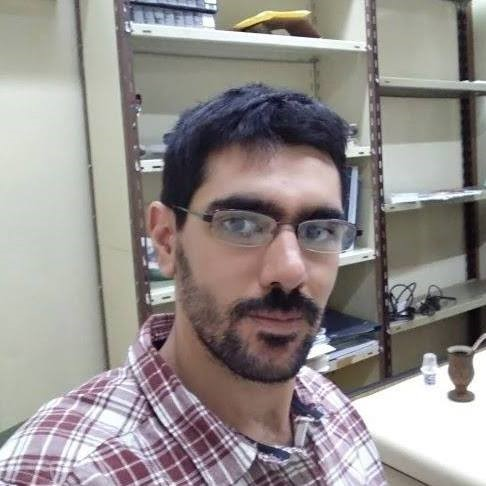
\includegraphics[width=1in,height=1.25in,clip,keepaspectratio]{./figures/AF.jpg}}]{Álvaro Luis Fraga}
 , born May 17, 1989, in Ciudad Autonoma de Buenos Aires, Argentina. He received his degree in Information System Engineering in 2014 from the Facultad Regional Tucuman, Universidad Tenológica Nacional. He is currently a PhD candidate at the Institute of Development and Design (INGAR), an institute of double dependence with the National Council of Scientific and Technical Research of Argentina (CONICET) and the Universidad Tecnológica Nacional, where he conducts research in the area of ontologies applied in industry and is a member and active volunteer for over 10 years in the IEEE Argentina section.
\end{IEEEbiography}
%\newpage
% if you will not have a photo at all:
\begin{IEEEbiography}[{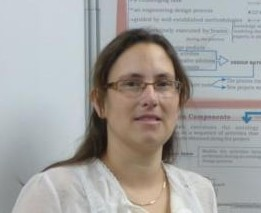
\includegraphics[width=1in,height=1.25in,clip,keepaspectratio]{./figures/MV.jpg}}]{Marcela Vegetti}
 is a professor at the Department of Information Systems Engineering of the Facultad Regional Santa Fe, Universidad Tecnológica Nacional (Santa Fe, Argentina). She also holds a position as assistant researcher at the National Council of Scientific and Technical Research of Argentina (CONICET), working at the "Instituto de Desarrollo y Diseño". She obtained her PhD. Degree in Engineering in Information Systems from Universidad Tecnológica Nacional in 2007. Her current research activities focus on the application of ontologies and semantic technologies for conceptual modeling and supporting interoperability in different domains.
\end{IEEEbiography}

% insert where needed to balance the two columns on the last page with
% biographies


\begin{IEEEbiography}[{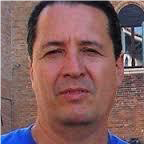
\includegraphics[width=1in,height=1.25in,clip,keepaspectratio]{./figures/HL.png}}]{Horacio Leone}
is a full Professor at the Department of Information Systems Engineering of the Facultad Regional Santa Fe, Universidad Tecnológica Nacional (Santa Fe, Argentina). He also holds a Researcher position at the National Council for Scientific and Technical Research of Argentina (CONICET), working at Instituto de Desarrollo y Diseño. He obtained his PhD degree in Chemical Engineering from Universidad Nacional del Litoral (Santa Fe, Argentina) in 1986 and was a Postdoctoral Fellow at the Massachusetts Institute of Technology (1986–1989). His current research activities focus on software architectures, models for supporting the design process, semantic web applications to supply chain information systems, and enterprise modelling. He has supervised several PhD students.
\end{IEEEbiography}

% You can push biographies down or up by placing
% a \vfill before or after them. The appropriate
% use of \vfill depends on what kind of text is
% on the last page and whether or not the columns
% are being equalized.

%\vfill

% Can be used to pull up biographies so that the bottom of the last one
% is flush with the other column.
%\enlargethispage{-5in}



% that's all folks
\end{document}


